\documentclass[a4paper]{article}

\usepackage[english]{babel}
\usepackage[utf8]{inputenc}
\usepackage{amsmath}
\usepackage{graphicx}
\usepackage[colorinlistoftodos]{todonotes}
\usepackage{makecell}
\usepackage{tikz} 
\usepackage{pgfplots}
\pgfplotsset{compat=1.8}
\usepackage{subcaption}
\usepackage{float}
\title{Automated bee wings classification : the Deepwings project}

\author{Théo Bodrito}

\date{December 21, 2018}

\begin{document}
\maketitle

\begin{abstract}
    Bees have been dying off at an extraordinary high rate, and no one is quite sure why. To investigate this issue, researchers need a quick and reliable way to identify bee species. This document introduces the Deepwings project, which compares deep learning and features extraction approaches to classify bee species from wings pictures.


\end{abstract}

\section{Introduction}
\label{sec:introduction}

About 35\% of the world's crops and 80\% of the world’s flowers are pollinated by bees! Most bees that are farmed for pollination are European Honeybees, whose physique and behavior makes them very efficient. But native bees can share in the pollination effort, and some may be more efficient.

Recently, honeybees have been dying off at an extraordinarily high rate, and no one is quite sure why. Researchers call it Colony Collapse Disorder, and the problem is serious because of our dependence on honeybees to pollinate food crops. While many are researching the cause of Colony Collapse Disorder, research into native bees may uncover more productive alternatives to the European honeybee. Finding the cause and potential native alternatives involve tracking wild bee populations and habits.

There are many species of bees, more than 500 in Wisconsin alone, but it's not easy to tell which species an individual belongs to.

While bee species identification is essential to research, identifying the species of a bee can be expensive and time-consuming. Since there are few experts who can reliably distinguish many different species, bees must be captured and sent to an expert, which may take several months. Bee research can be excruciatingly slow.

Rather than capturing, killing, and sending the bees off to be catalogued, imagine an iPhone app that lets graduate students and researchers identify bees in the field. One could simply take a photo of a bee and instantly record its species and location. Research could be conducted much faster, and identified bees could be released back to nature.


\section{Previous work in bee wings identification}
\label{sec:theory}

We relied mostly on Christopher Hall's work for features extraction: \textit{An Automated Approach to Bee Identification from Wing Venation} (2011).

\section{Dataset}
The initial dataset was composed of 1193 images, but we cleaned it so as to have at least 20 images per species.
So the dataset we used consists of 1135 images belonging to different genera, and each genus is divided into different species as follows :

\begin{figure}[h]
    \begin{tabular}{ |m{2cm}|m{10em}|m{10em}| }
 \hline
genus & species & Number of images \\
\hline
bombus& \makecell{impatiens \\ griseocolis \\ ...}& \makecell{65  \\ 26 \\...}\\
\hline
osmia & \makecell{ribifloris \\ lignaria \\ ...}  & \makecell{61\\ 58\\ ...}\\
\hline
\makecell{agapostemon \\ ... }& \makecell{texanus \\ ...}& \makecell{107  \\... }\\
\hline
5 genera & 21 species & 1135 images\\
\hline
\end{tabular}
\caption{Dataset structure}
\end{figure}


\begin{figure}[h]
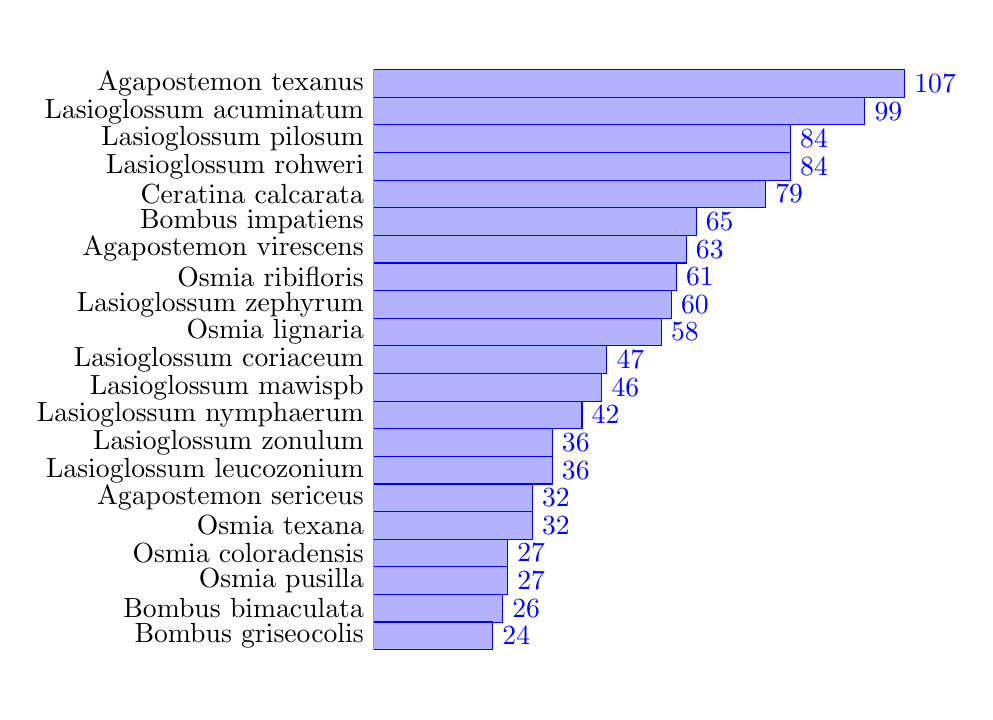
\begin{tikzpicture}
\begin{axis}[ 
xbar, xmin=0,
tickwidth=0pt,
y axis line style = { opacity = 0 },
height=10cm,width=9cm,
xlabel={Percentage },
axis x line=none,
symbolic y coords={
{Bombus griseocolis},
{Bombus bimaculata},
{Osmia pusilla},
{Osmia coloradensis},
{Osmia texana},
{Agapostemon sericeus},
{Lasioglossum leucozonium},
{Lasioglossum zonulum},
{Lasioglossum nymphaerum},
{Lasioglossum mawispb},
{Lasioglossum coriaceum},
{Osmia lignaria},
{Lasioglossum zephyrum},
{Osmia ribifloris},
{Agapostemon virescens},
{Bombus impatiens},
{Ceratina calcarata},
{Lasioglossum rohweri},
{Lasioglossum pilosum},
{Lasioglossum acuminatum},
{Agapostemon texanus}
},
ytick=data,
nodes near coords, 
nodes near coords align={horizontal},
ytick=data,
]
\addplot coordinates {
(24,{Bombus griseocolis})
(26,{Bombus bimaculata})
(27,{Osmia pusilla})
(27,{Osmia coloradensis})
(32,{Osmia texana})
(32,{Agapostemon sericeus})
(36,{Lasioglossum leucozonium})
(36,{Lasioglossum zonulum})
(42,{Lasioglossum nymphaerum})
(46,{Lasioglossum mawispb})
(47,{Lasioglossum coriaceum})
(58,{Osmia lignaria})
(60,{Lasioglossum zephyrum})
(61,{Osmia ribifloris})
(63,{Agapostemon virescens})
(65,{Bombus impatiens})
(79,{Ceratina calcarata})
(84,{Lasioglossum rohweri})
(84,{Lasioglossum pilosum})
(99,{Lasioglossum acuminatum})
(107,{Agapostemon texanus})
};
\end{axis}
\end{tikzpicture} %width=6cm,height=7.59cm
\caption{Number of images per species}
\end{figure}

\vspace{10cm}
\section{First method : CNN}
Convolutional Neural Networks are best suited for image classification. 
We compared two different architectures: VGG16 and DenseNet121.

\subsection{VGG16}
This model came out in 2014. It is a very deep and very classical CNN base folowed by 3 Dense layers.
It achieved great performance at the time, but one of its biggest flaw is its size: it can be very difficult to train it from scratch.

\begin{figure}[h]
    \centering
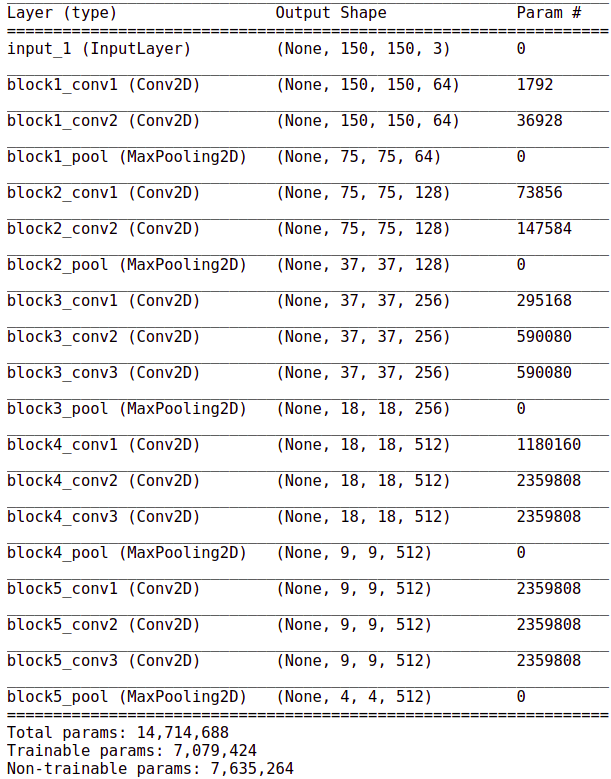
\includegraphics[width=.6\textwidth]{figures/architecture_vgg16.png}
\caption{Architecture base VGG16}
\end{figure}

Our dataset was not big enough, that's why we had to use \textit{transfer learning} : the idea is to use a pretrained convolutional base (trained on imagenet).
The first step is to train the top layers (the dense ones) while the weigths of the base remain frozen. Then, we defreeze the top 3 layers of the  convolutional base, to fit our dataset more precisely. This last step is called \textit{fine tuning}.

\begin{figure}[h]
    \centering
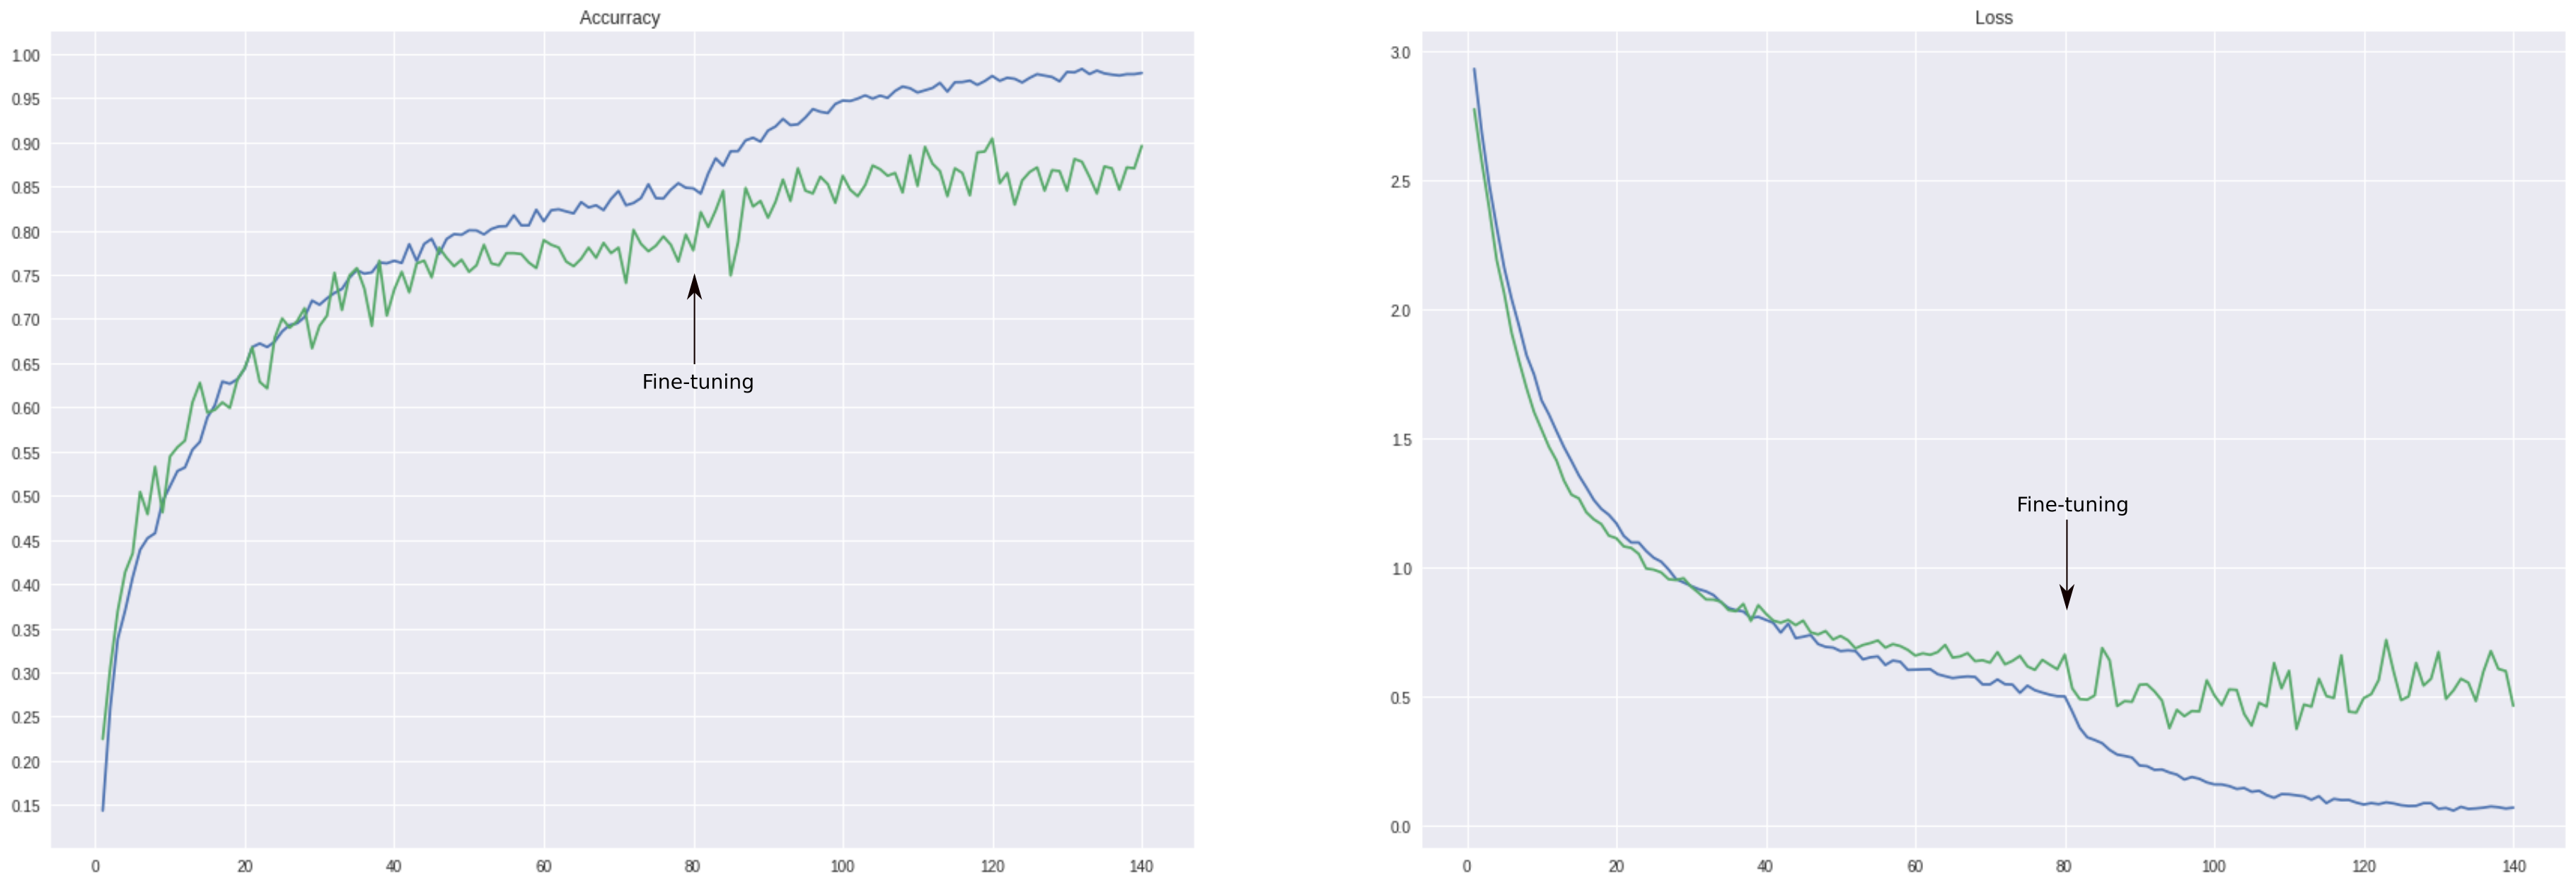
\includegraphics[width=.8\textwidth]{figures/vgg16_graph_caption.png}
\caption{VGG16 training with fine-tuning}
\end{figure}

\newpage
\subsection{DensetNet121}
DensNets came out in 2016. 
This model is lighter than VGG16 and faster to train than VGG16 thanks to shorter connections between layers: each layer is connected to every other layer in a feed-forward fashion. 

\begin{figure}[h]
    \centering
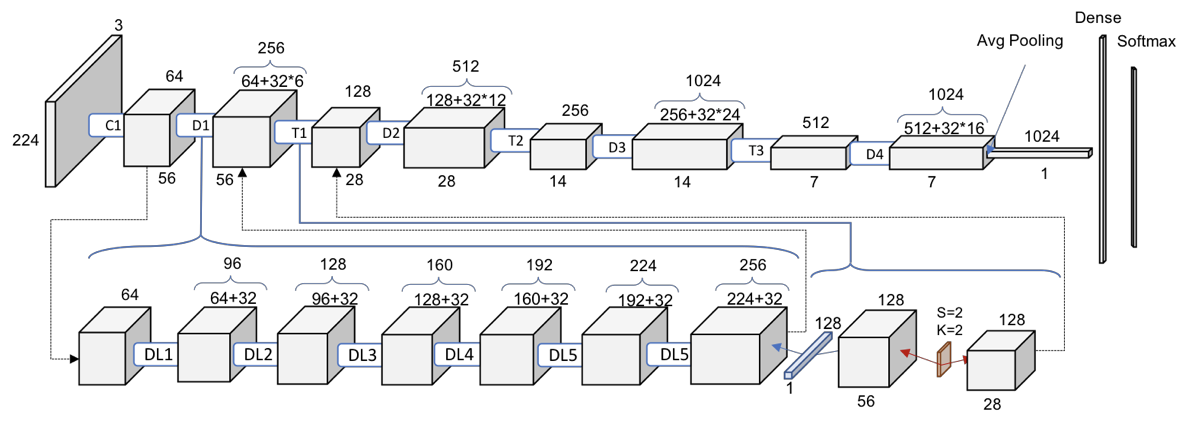
\includegraphics[width=.8\textwidth]{figures/densenet121_architecture.png}
    \caption{Architecture DenseNet121}
\end{figure}

\begin{figure}[h]
    \centering
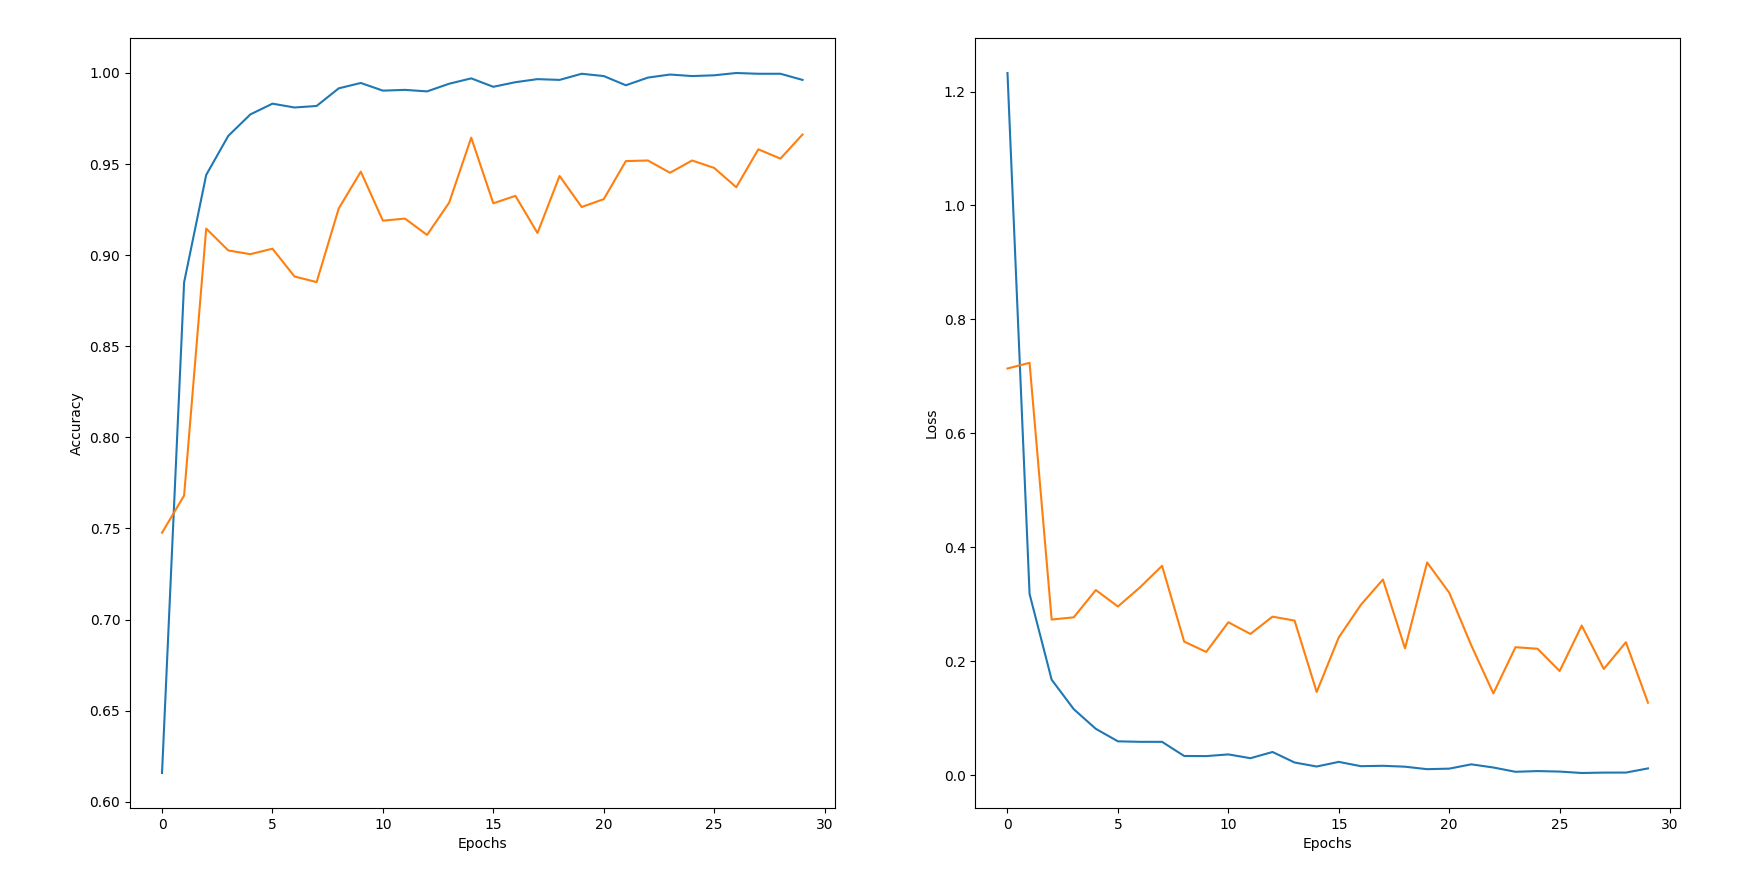
\includegraphics[width=.8\textwidth]{figures/graph_densenet.png}
    \caption{DenseNet121 training (without fine-tuning)}
\end{figure}

As you can see on the curves, DenseNet121 reaches better accuracy than VGG16 on the same dataset (95\% vs 88\%).
Furthermore, its light weight make it the perfect CNN model for our project.


\section{Second method : Features extraction}

\subsection{Bee wings cells}

Bee wings are divided into several cells :

\begin{figure}[h]
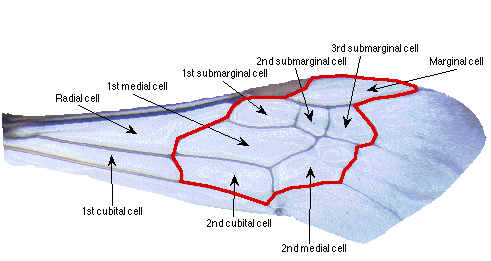
\includegraphics[width=.8\textwidth]{figures/schema_wings2.png}
\caption{Cells names}
\end{figure}

The cells we are interested in are circled in red. Those cells were chosen because they are entirely visible on all images from the dataset. Nevertheless we need to be careful because the 3rd submarginal cell is not always separated from the 2nd submarginal cell, it depends on the species. We have to keep that in mind for the next steps.

First of all, we need to detect those cells, then we have to identify them and finally, extract features from them.
\newpage
\subsection{Regions detection}

\subsubsection{Binarizations}
The first step is to binarize the image so as to detect the veins and cells clearly. To do that, we compute a grayscale image and then we compare the value of each pixel to a threshold. If the value is above the threshold, it becomes "True" or white in the binarized image, otherwise it turns black or "False". This threshold can be global :
\begin{itemize}
    \item Global : unique threshold for all pixels.
    \item Local : different thresholds for different part of the image. It allows for a more refined binary image, and it helps discarding variation of shades in the input image.
\end{itemize}

\begin{figure}[H]
\centering
\begin{subfigure}{.35\textwidth}
  \centering
    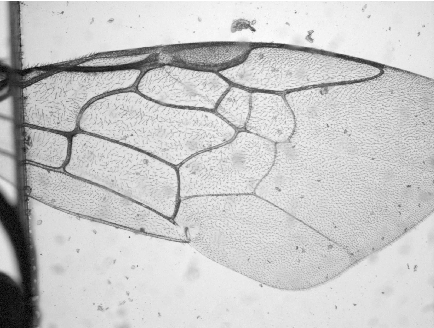
\includegraphics[width=\linewidth]{figures/original.png}
    \caption{Original}
\end{subfigure}
\begin{subfigure}{.35\textwidth}
  \centering
  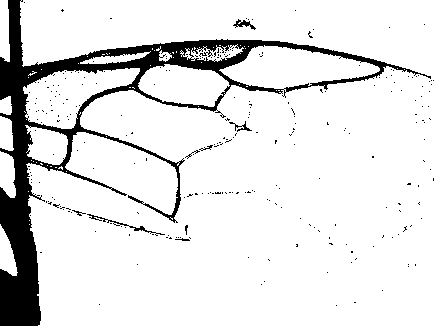
\includegraphics[width=\linewidth]{figures/otsu.png}
  \caption{Otsu}
\end{subfigure}

\begin{subfigure}{.35\textwidth}
  \centering
  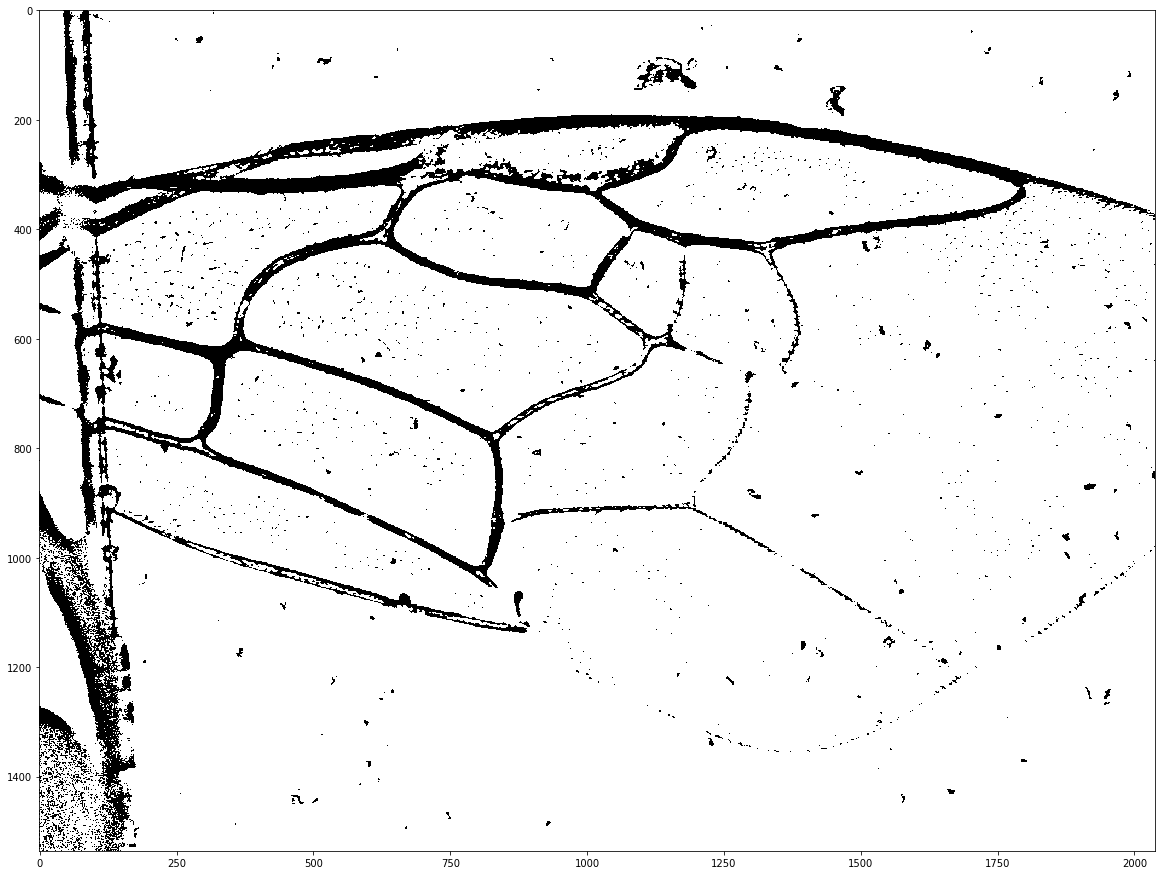
\includegraphics[width=\linewidth]{figures/niblack.png}
  \caption{Niblack}
\end{subfigure}
\begin{subfigure}{.35\textwidth}
  \centering
  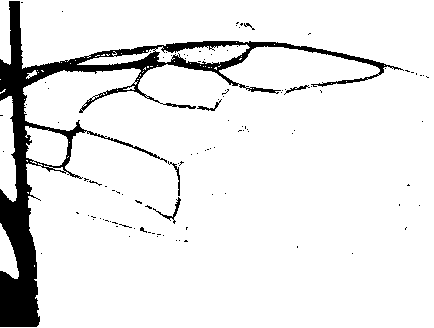
\includegraphics[width=\linewidth]{figures/minimum.png}
  \caption{Minimum}
\end{subfigure}

\begin{subfigure}{.35\textwidth}
  \centering
    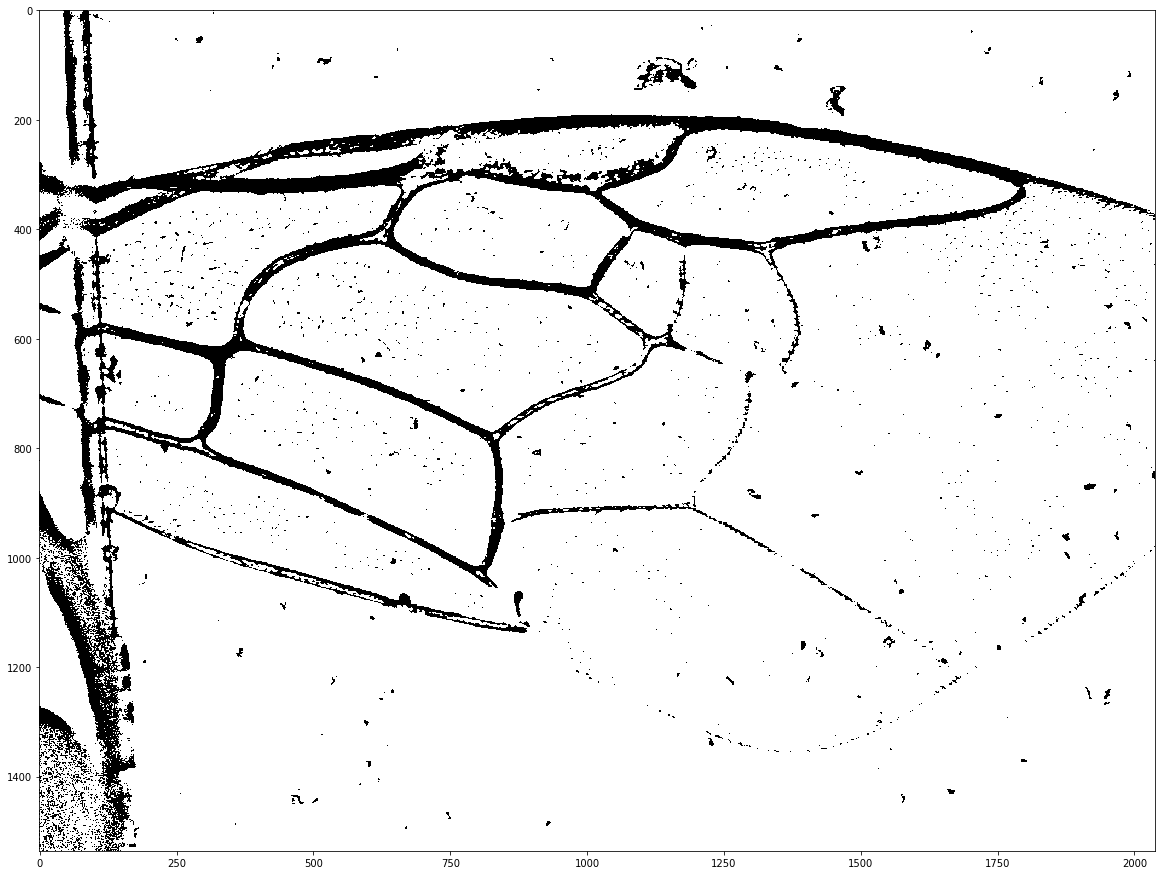
\includegraphics[width=\linewidth]{figures/sauvola.png}
    \caption{Sauvola}
\end{subfigure}
\begin{subfigure}{.35\textwidth}
  \centering
    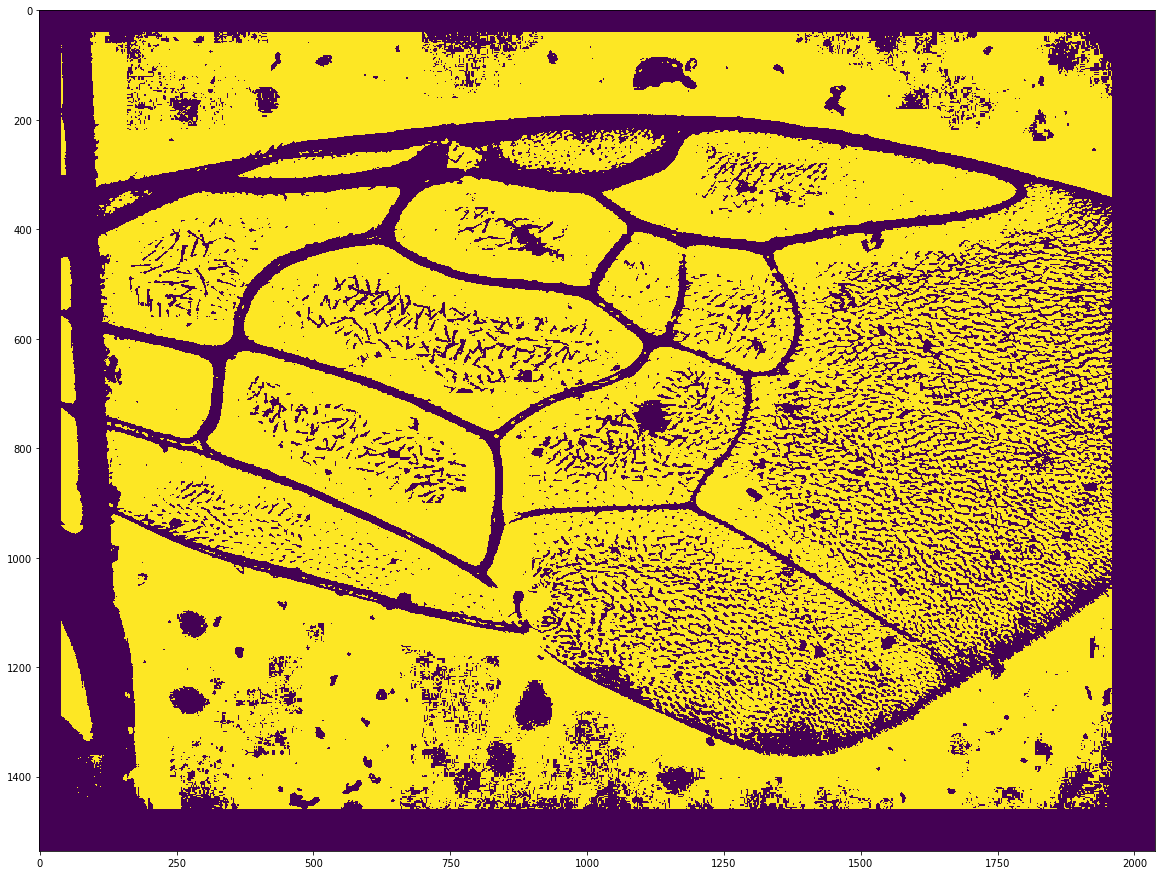
\includegraphics[width=\linewidth]{figures/blocks.png}
    \caption{Blocks binarization}
\end{subfigure}
    \caption{Different binarizations: global (\textit{b, d}) vs local (\textit{c, e, f}) thresholds}
\label{binarizations}
\end{figure}

As shown in figure \ref{binarizations} veins are better segmented with local thresholds, and especially with blocks binarization (ref Chris Hall). In other cases, the veins are not complete which will be an issue in the following steps.
\newpage
\subsubsection{Blocks binarization}

The idea here is to divide the input image into blocks and binarize each block independently with Otsu binarization to obtain a "sub-binarization". We repeat the process with different overlapping grids, and then sum all the "sub-binarizations" to obtain a grayscale image, to which we apply one last global Otsu binarization. 
The technique results in the binary image shown in figure \ref{blocks_binarization}.

\begin{figure}[H]
\begin{subfigure}{.5\textwidth}
    \centering
    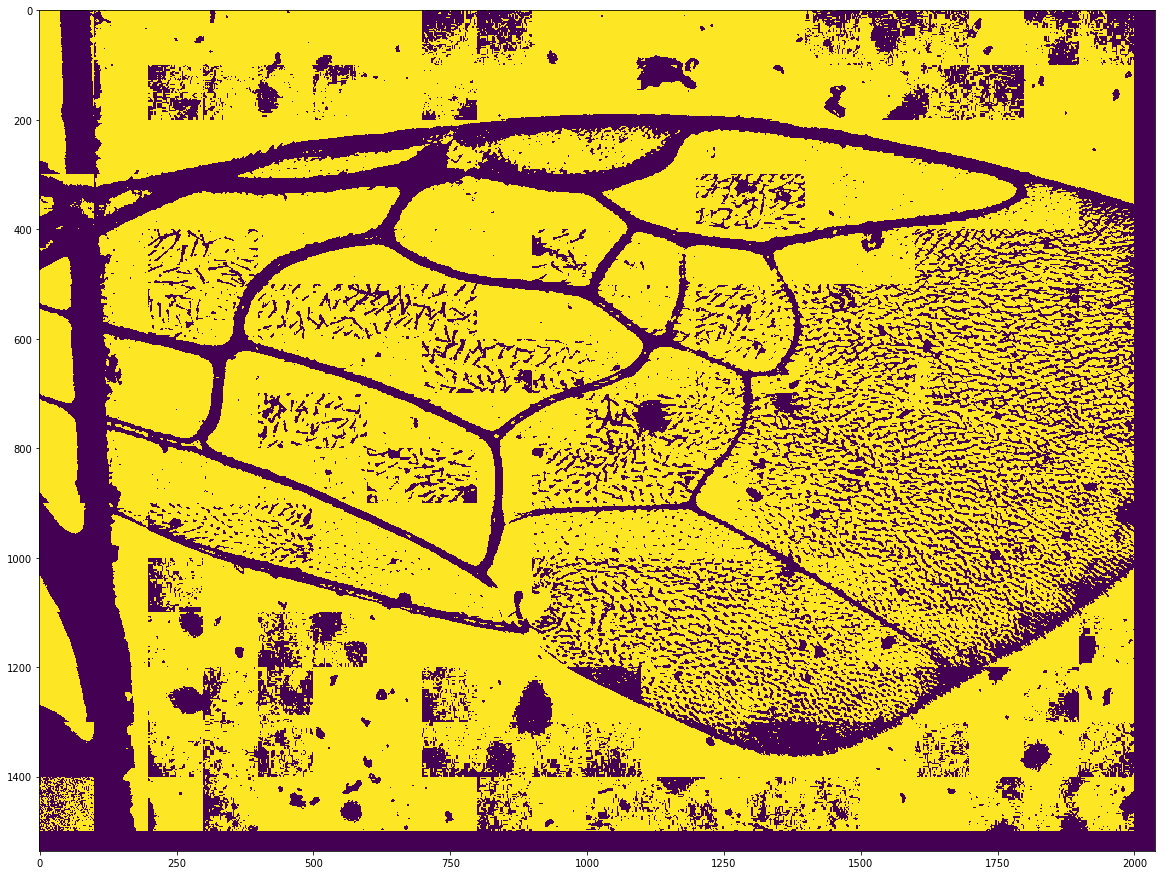
\includegraphics[width=\textwidth]{figures/sub_blocks.png}
    \caption{sub-binarization 1}
\end{subfigure}
\begin{subfigure}{.5\textwidth}
    \centering
    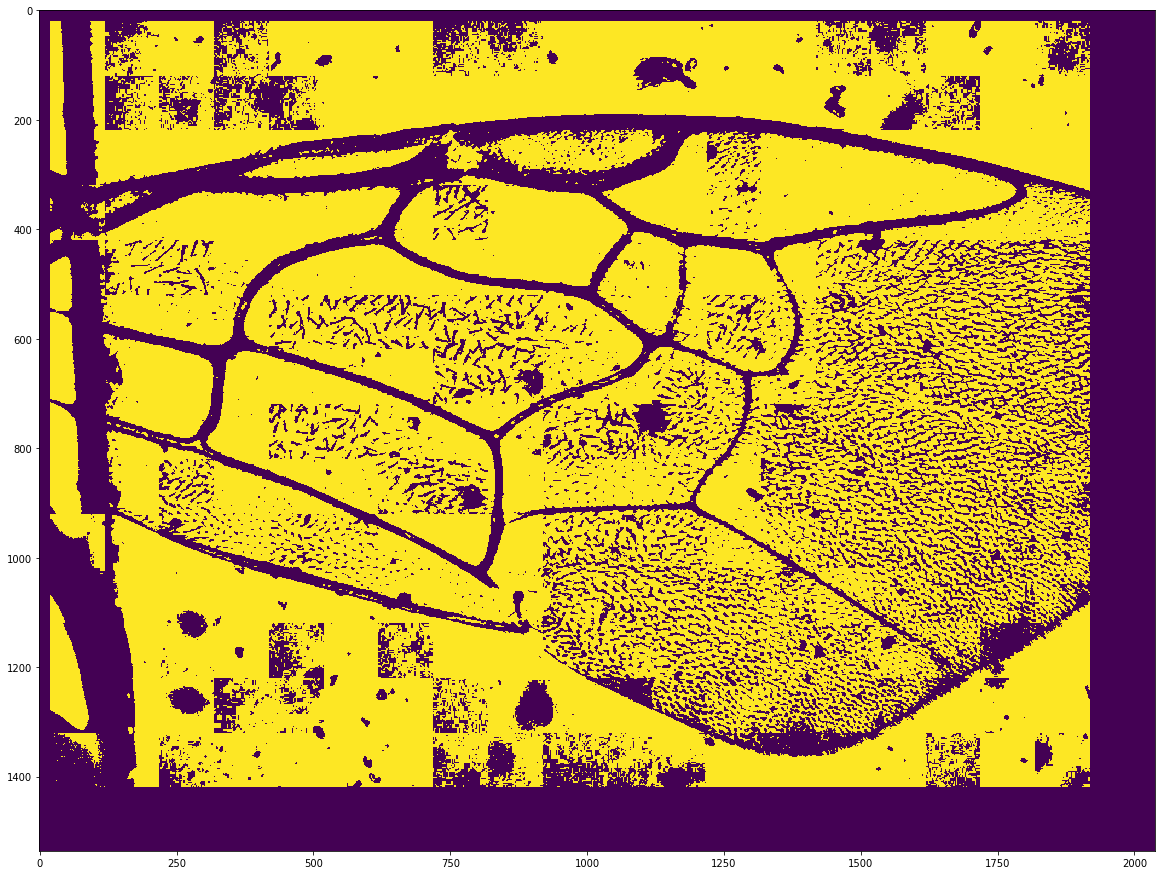
\includegraphics[width=\textwidth]{figures/sub_blocks2.png}
    \caption{sub-binarization 2}
\end{subfigure}
\begin{subfigure}{.5\textwidth}
    \centering
    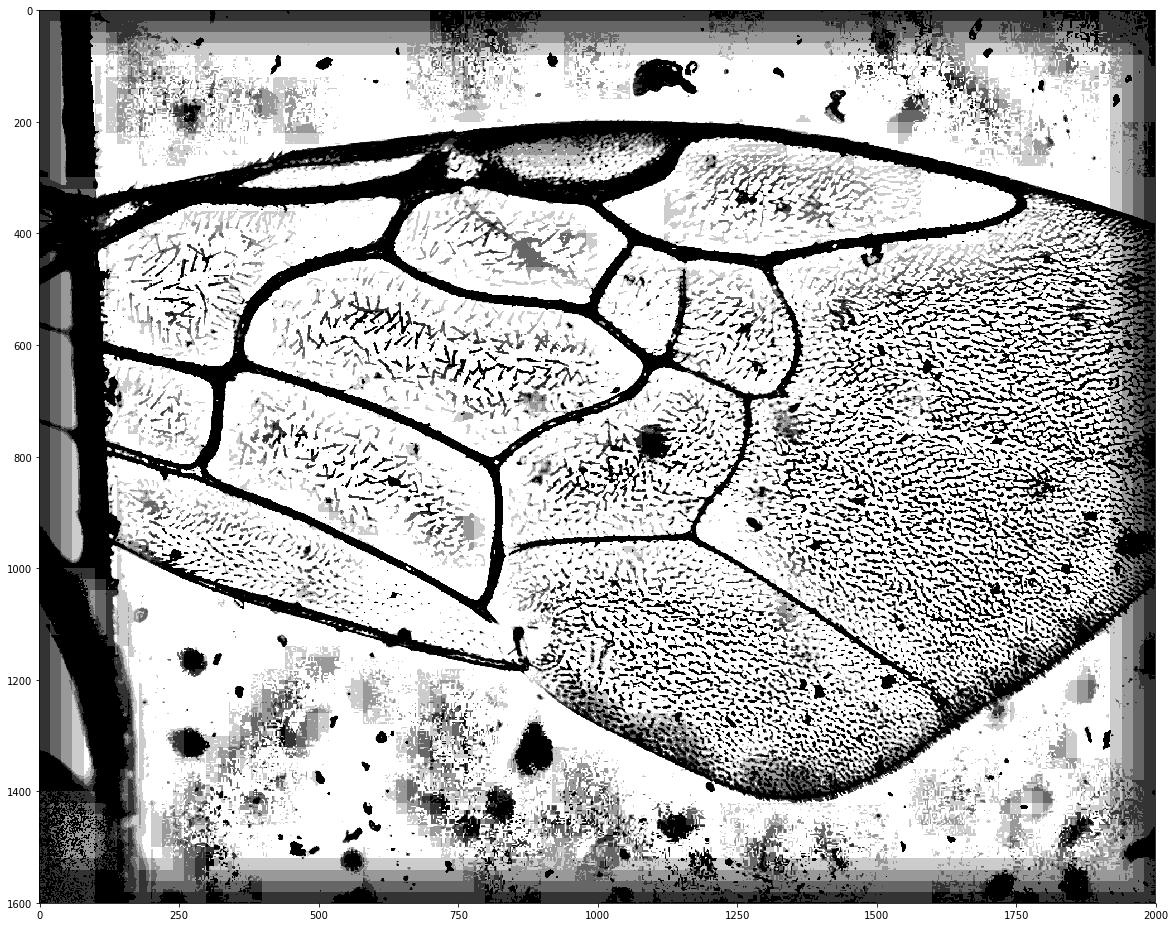
\includegraphics[width=\textwidth]{figures/sum_blocks_bin.png}
    \caption{Sum of all sub-binarizations}
\end{subfigure}
\begin{subfigure}{.5\textwidth}
    \centering
    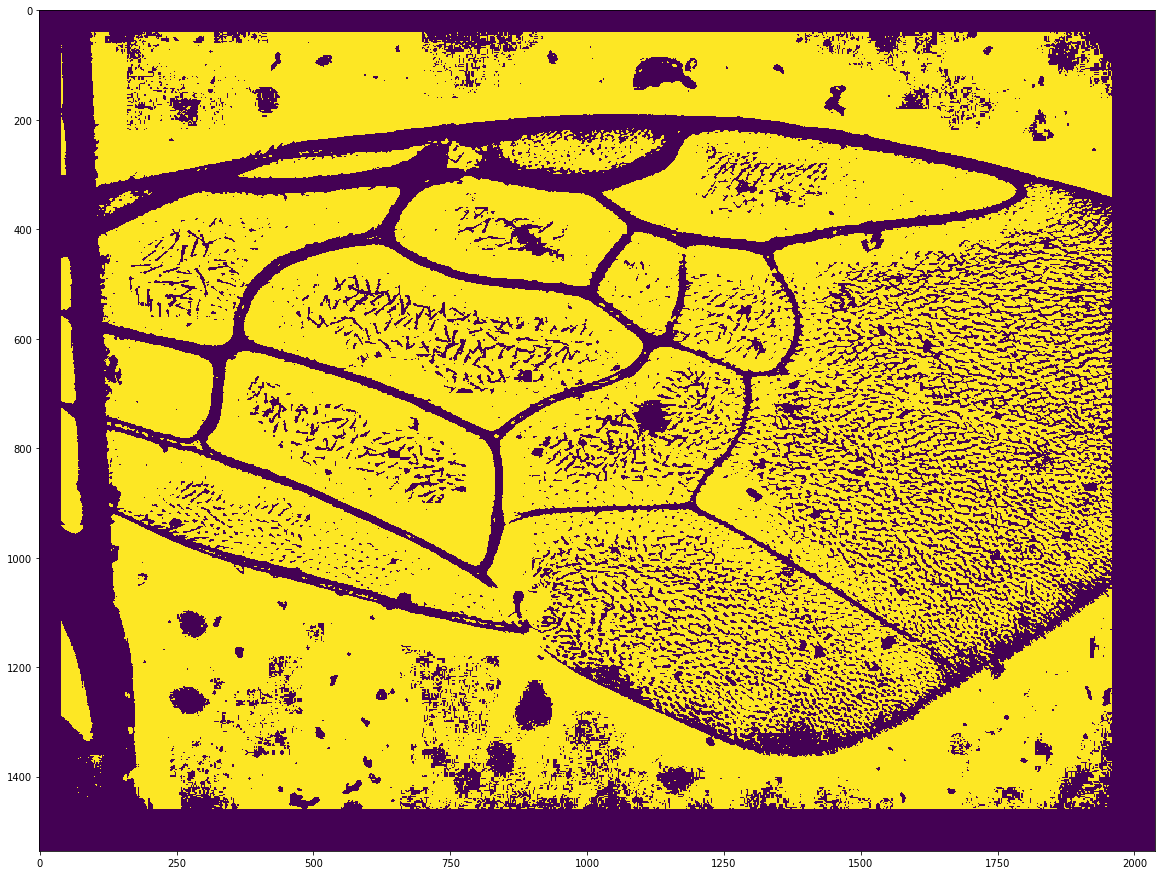
\includegraphics[width=\textwidth]{figures/blocks.png}
    \caption{Final binarized image}
\end{subfigure}
\caption{Blocks binariation : step by step}
\label{blocks_binarization}
\end{figure}

The advantage of using overlapping grids is to overcome border effects : taken independently, sub-binarizations 1 and 2 in figure \ref{blocks_binarization} are not sufficient to clear the veins, but when combined, the binary image is much more refined.\\
At this stage, still having hairs inside the cells is not an issue. They will be removed in the next step.

\subsubsection{Post processing}

\begin{figure}[H]

    \begin{subfigure}[t]{.5\textwidth}
    \centering
    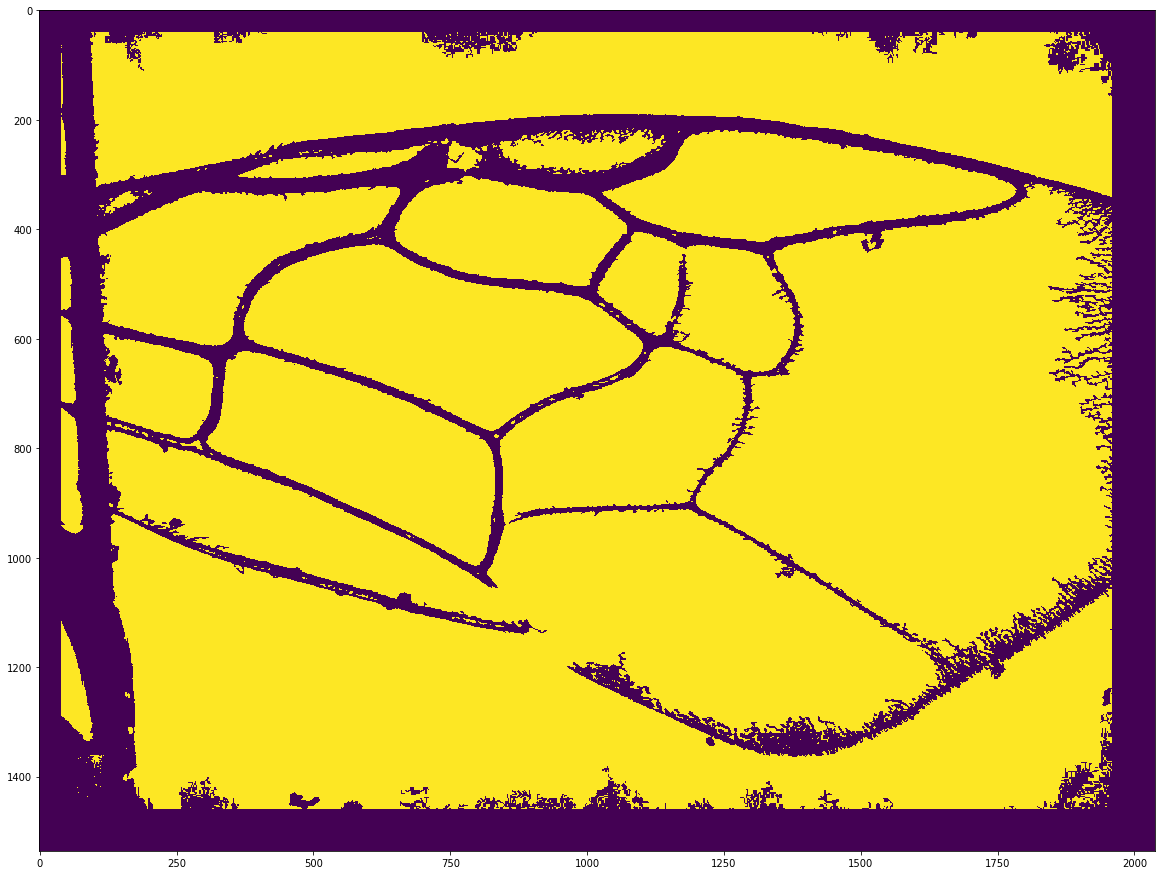
\includegraphics[width=\textwidth]{figures/cleared.png}
    \caption{Morphological reconstruction by erosion}
\end{subfigure}
    \begin{subfigure}[t]{.5\textwidth}
    \centering
    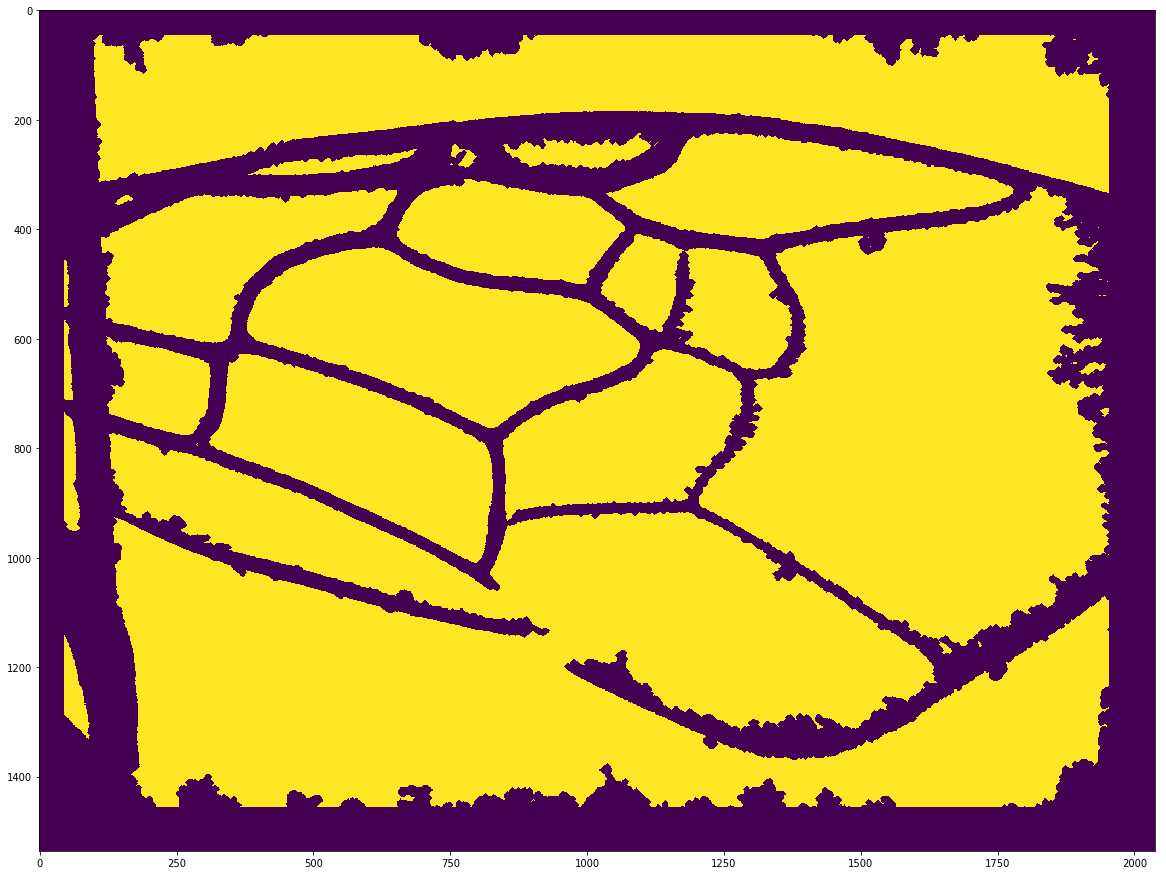
\includegraphics[width=\textwidth]{figures/eroded.png}
    \caption{Binary erosion}
\end{subfigure}
\caption{Post-processing}
\label{postprocessing}
\end{figure}

Now we need to remove the remaining hairs inside the cells. To do that, we use morphological reconstruction by erosion : it removes all black pixels not connected to the border of the frame. This way, veins are preserved and cleared. In order to reinforce veins, we use binary dilation on top of that (see figure \ref{postprocessing}).

\subsubsection{Labels}
Now that all veins are detected, we want to separate the different regions in order to detect cells. We attribute labels (ie. integer values) to those regions in order to refer to them.

\begin{figure}[H]

    \begin{subfigure}[t]{.5\textwidth}
    \centering
    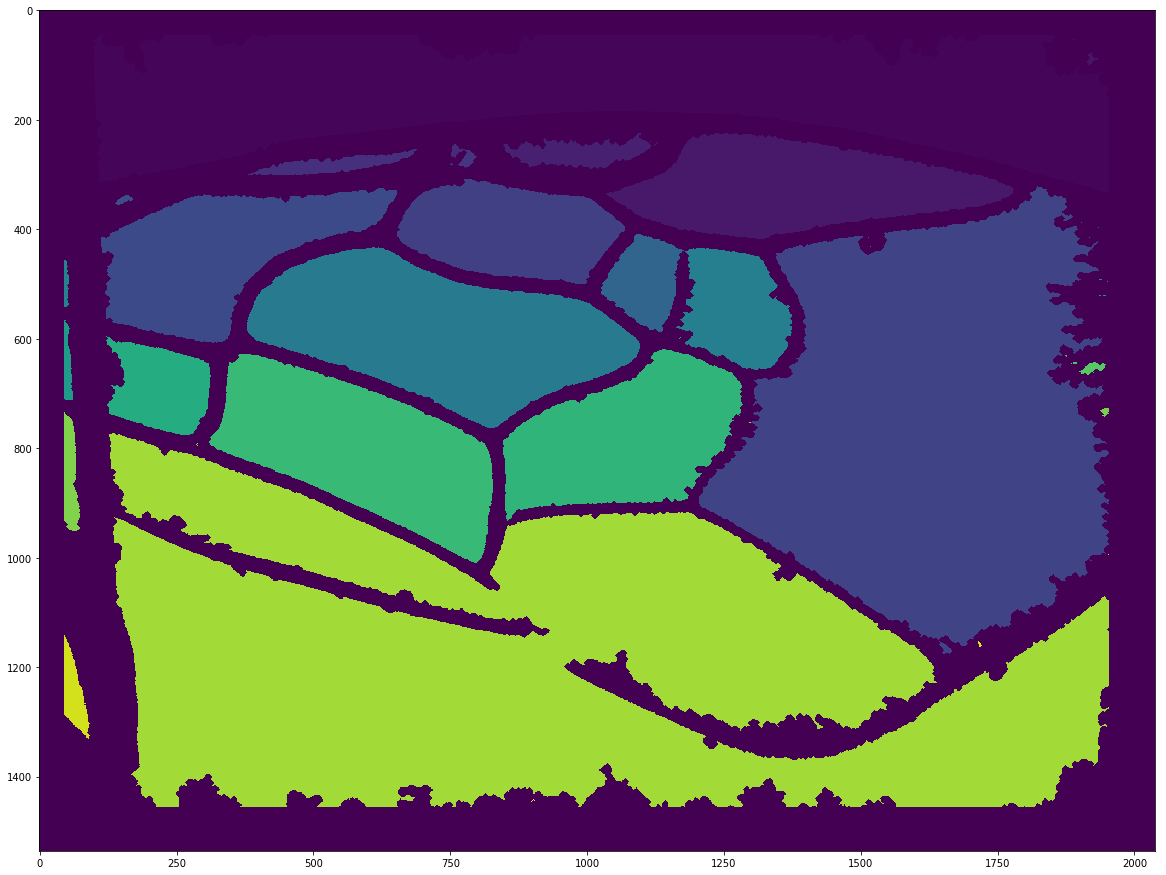
\includegraphics[width=\textwidth]{figures/markers1.png}
    \caption{Labelized image}
\end{subfigure}
    \begin{subfigure}[t]{.5\textwidth}
    \centering
    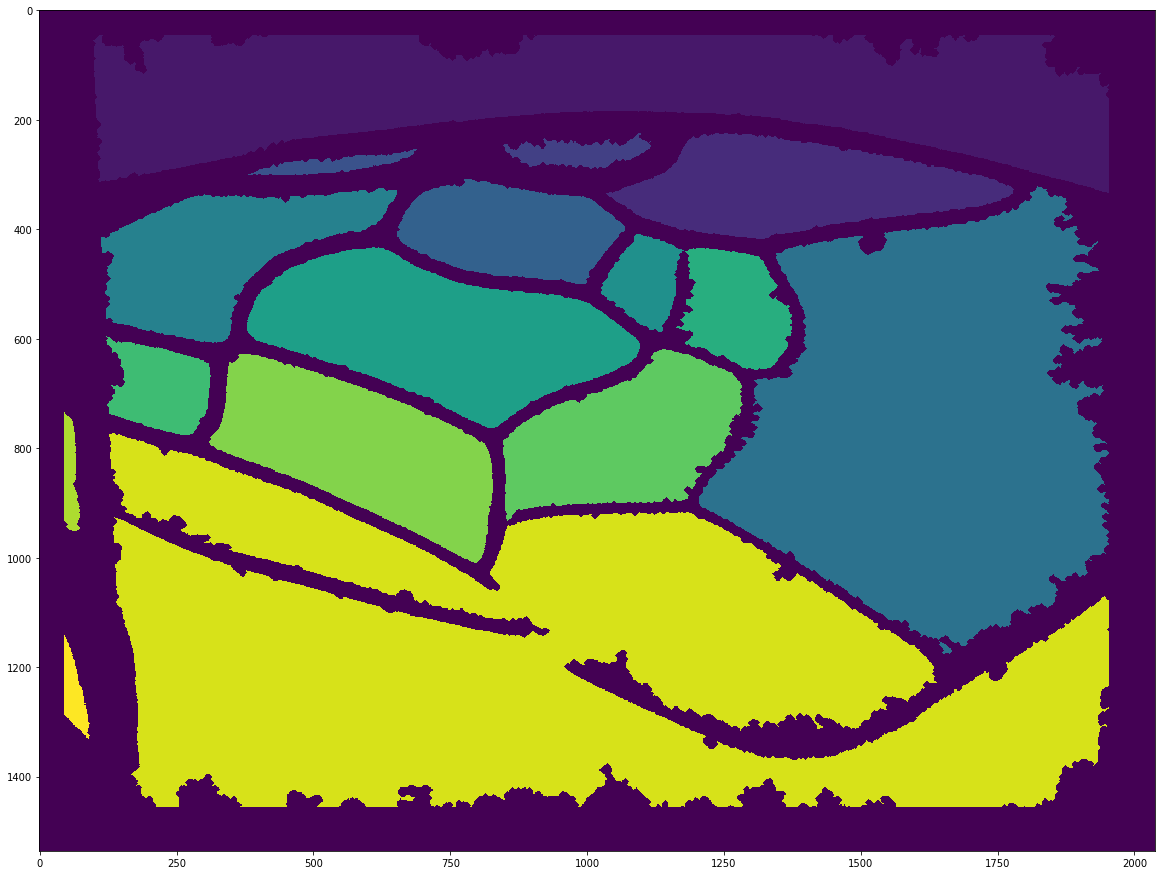
\includegraphics[width=\textwidth]{figures/markers2.png}
    \caption{Small regions discarded}
\end{subfigure}
\caption{Labels}
\label{labels}
\end{figure}

Then we discard small regions as they they might cause trouble in the next stages (see figure \ref{labels}).

\subsubsection{Watershed}

Now we have regions, but their edges are not ivery well defined because of the binary dilation done before. To improve accuracy on the edges, we use watershed segmentation. To do so, we first need to compute a distance map of our binary image : for each pixel of the foreground, we compute the shortest distance to a background pixel.  

\begin{figure}[h]
\begin{subfigure}{.4\textwidth}
  \centering
    \begin{subfigure}{\textwidth}
    \centering
        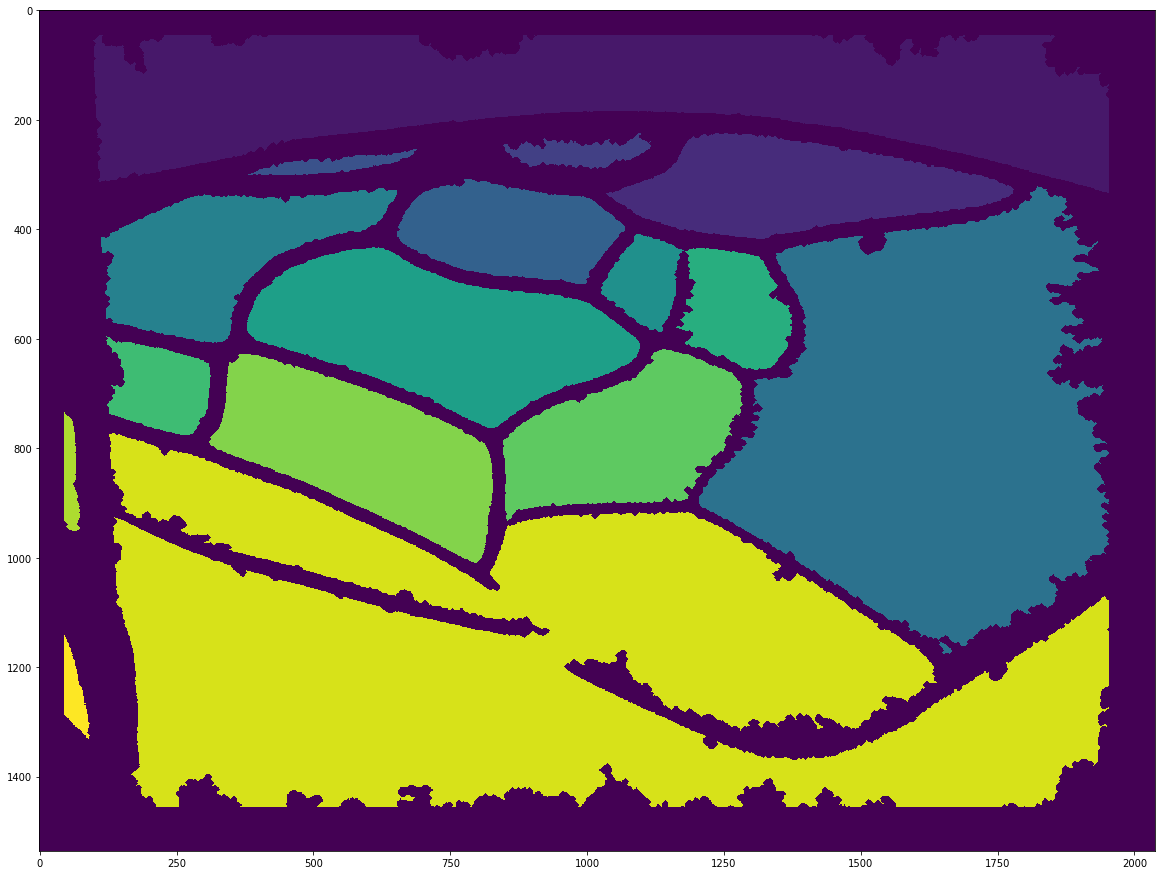
\includegraphics[width=\linewidth]{figures/markers2.png}
        \caption{Labels}
    \end{subfigure}\\
    \begin{subfigure}{\textwidth}
    \centering
        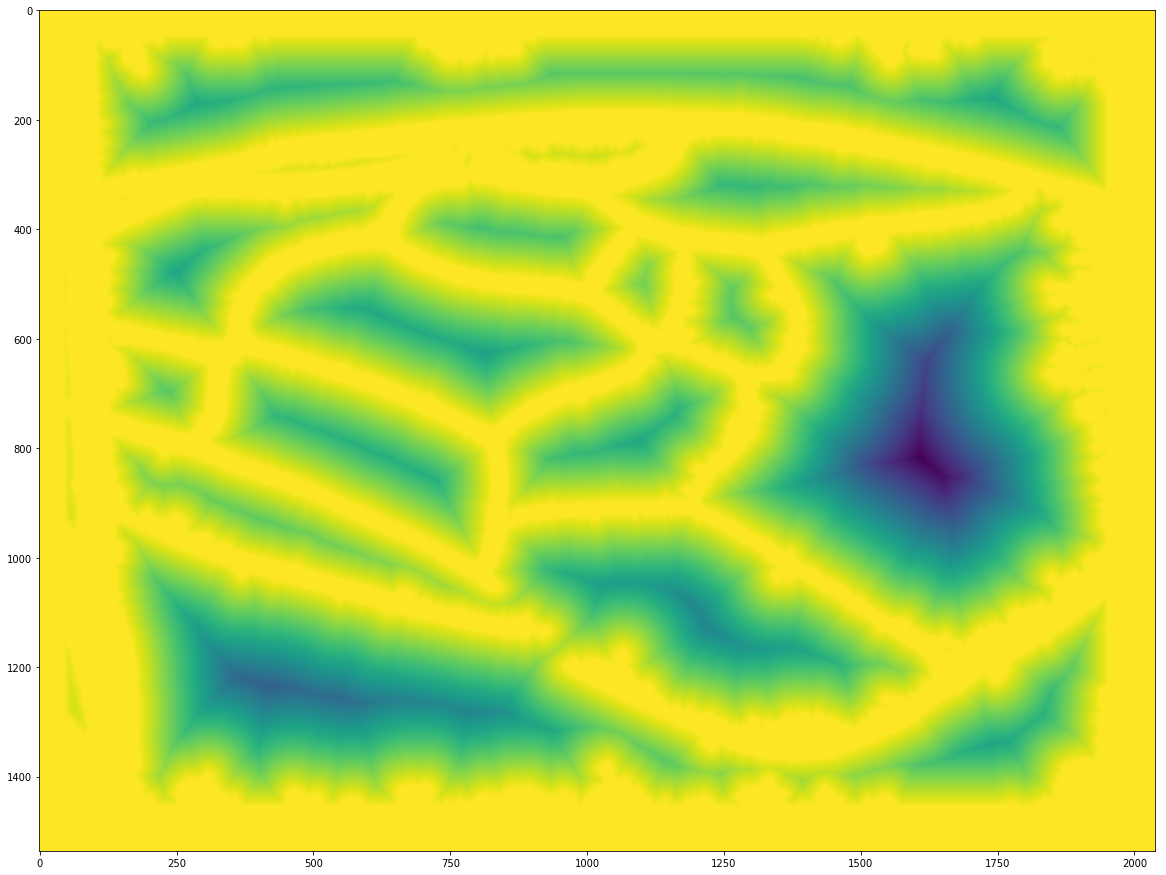
\includegraphics[width=\linewidth]{figures/distances.png}
        \caption{Distance map (reversed)}
    \end{subfigure}
\end{subfigure}
  \centering
\begin{subfigure}{.5\textwidth}
    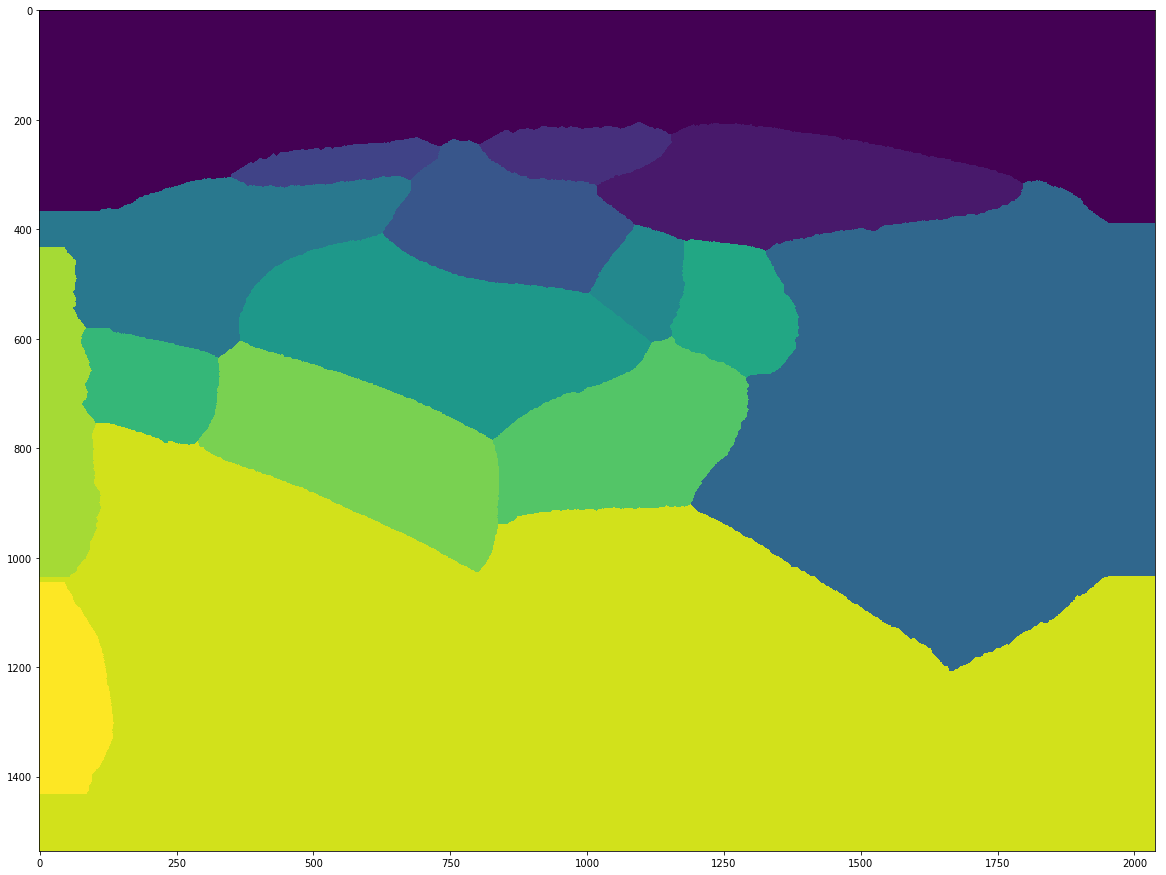
\includegraphics[width=\linewidth]{figures/watershed.png}
    \caption{After watershed segmentation}
\end{subfigure}
        
\caption{Watershed segmentation}
\end{figure}


We use both markers (labels) and reversed distance map to compute the watershed segmentation. We have now a much more refined description of our regions. This will be useful to filter them. 

\subsubsection{Clear borders}

As the regions we are interseted in (ie. the cells previously described) are located at the center of the image, we discard all regions in direct contact with the top, left and bottom borders of the frame. 
We don't remove regions adjacent to the right border because it happens sometimes with the marginal cell, which we wan to keep absolutely.

\begin{figure}[H]
    \centering
    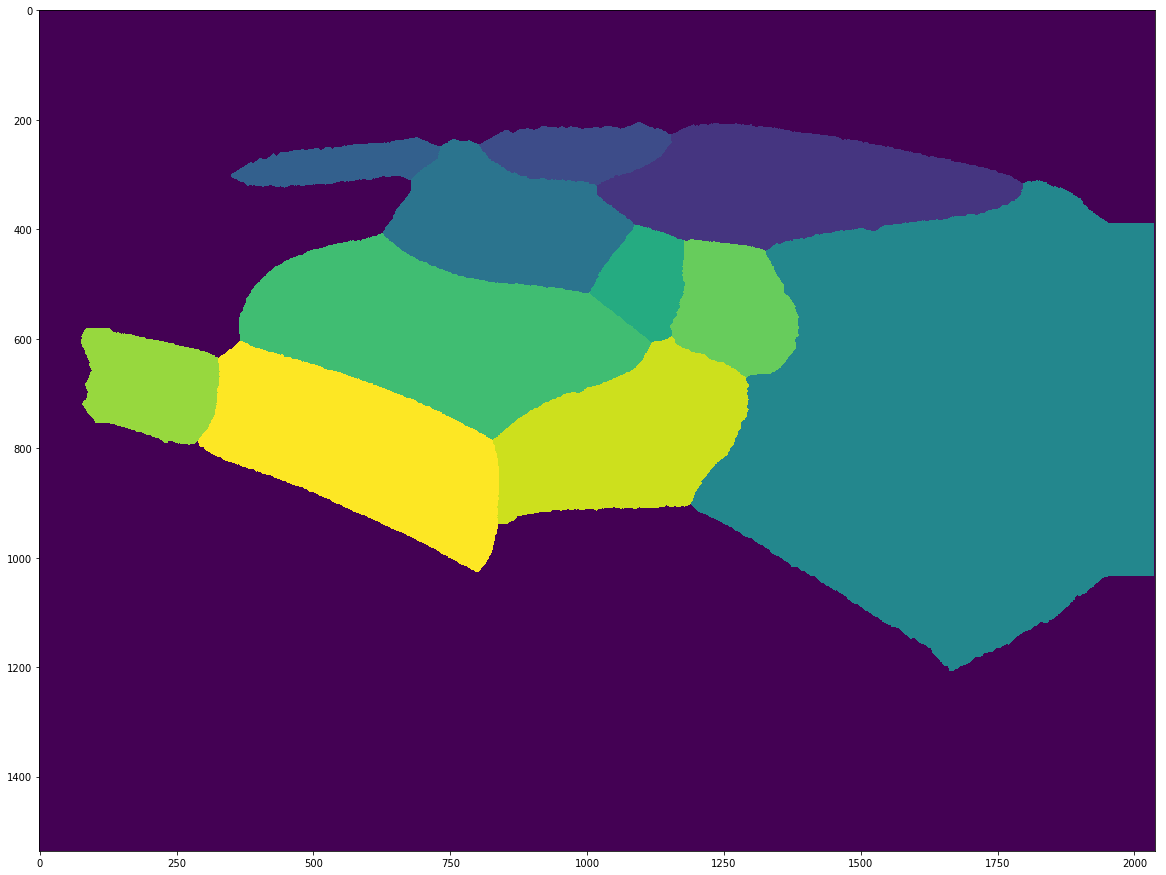
\includegraphics[width=.6\textwidth]{figures/clear_borders.png}
    \caption{Clear borders}
\end{figure}

\newpage
\subsection{Regions filtering}

Now that we have roughly detected the regiosn of interest, we are going to refine this selections through a set of filters.

\subsubsection{Area filter}

The first filter discard regions based on their area. It uses a threshold proportionate to the area of the whole image.

\begin{figure}[H]
\begin{subfigure}{.5\textwidth}
    \centering
    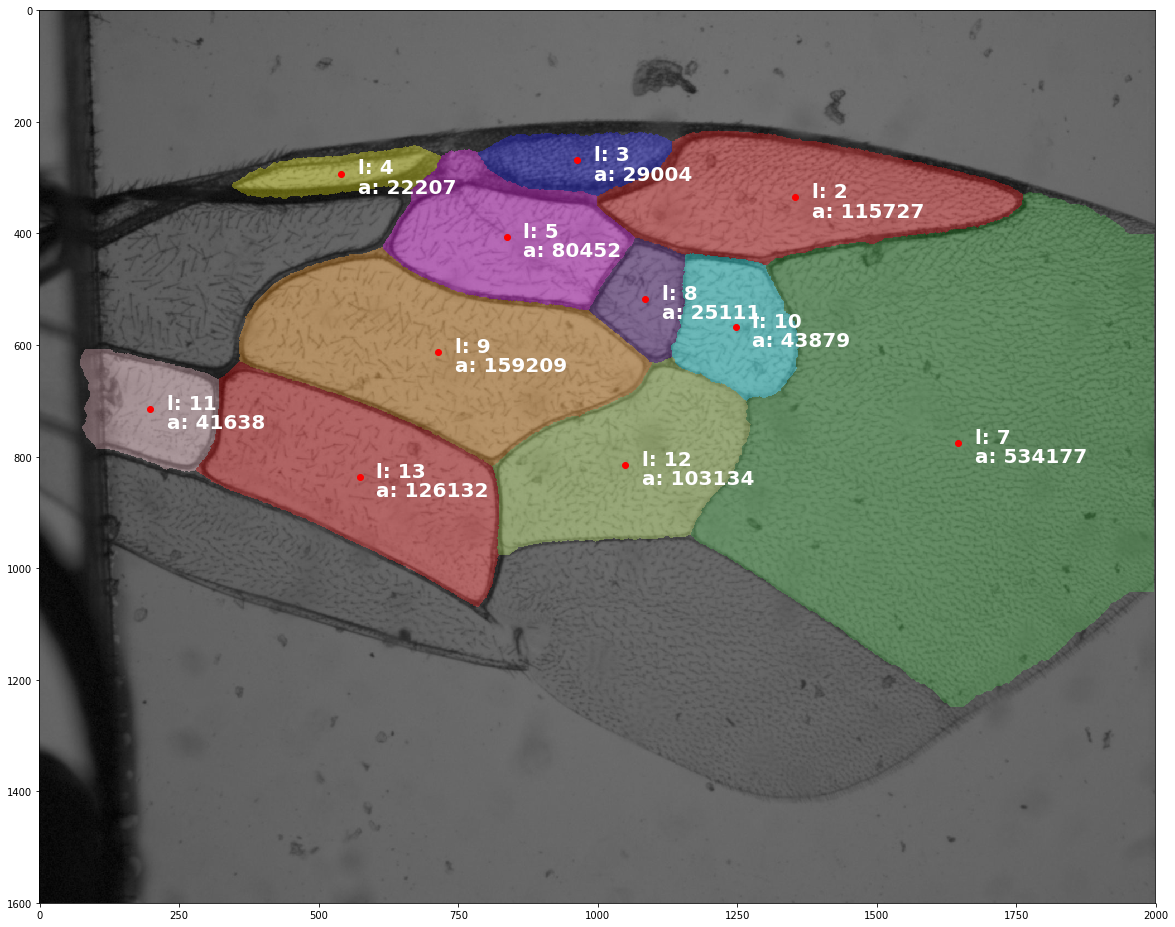
\includegraphics[width=\linewidth]{figures/first_rs.png}
    \caption{Before filtering}
\end{subfigure}
\begin{subfigure}{.5\textwidth}
    \centering
    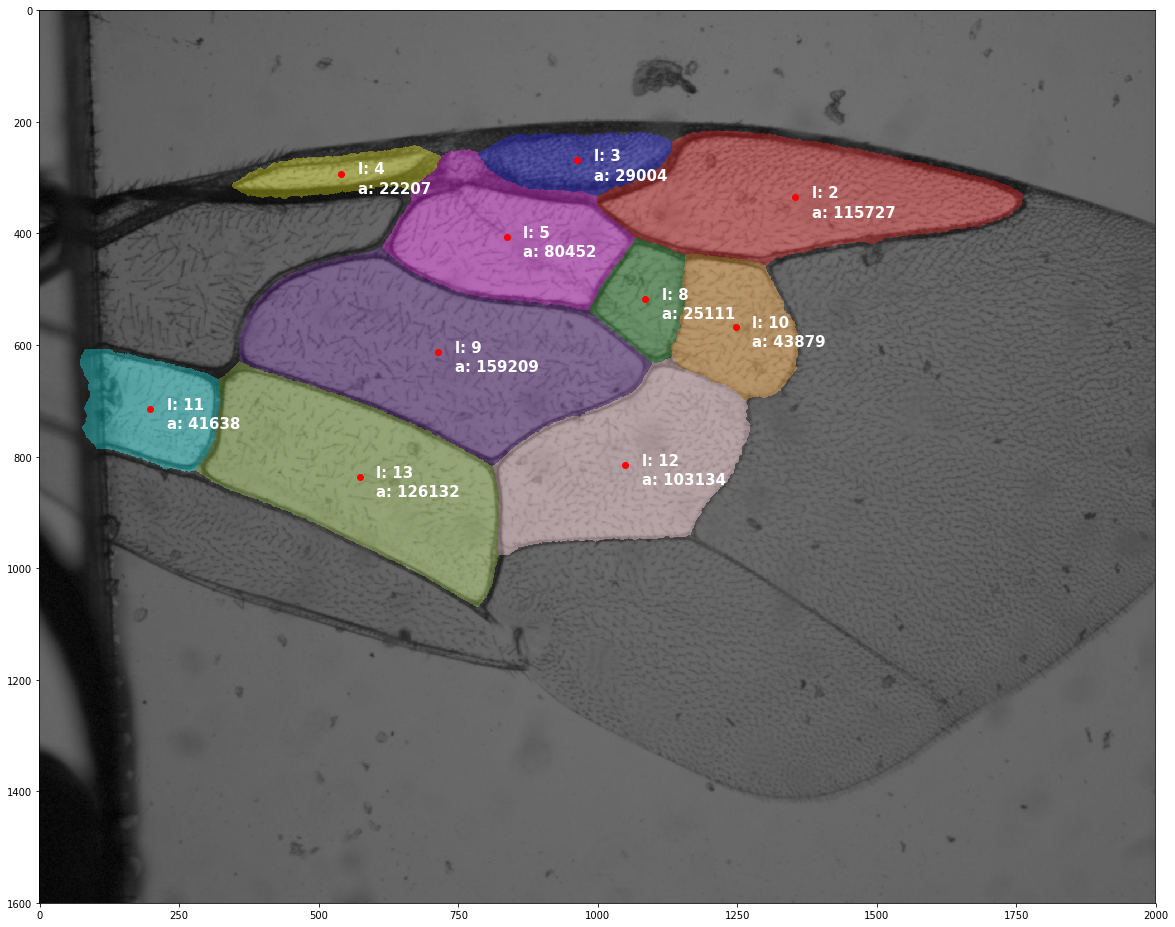
\includegraphics[width=\linewidth]{figures/filter_area.png}
    \caption{Area filter}
\end{subfigure}
\caption{Area filter}
\end{figure}

\subsubsection{Neighbors filter}
We determine each region's neighbors, and we discard those having less than 2 neighbors. 


\begin{figure}[H]
    \centering
    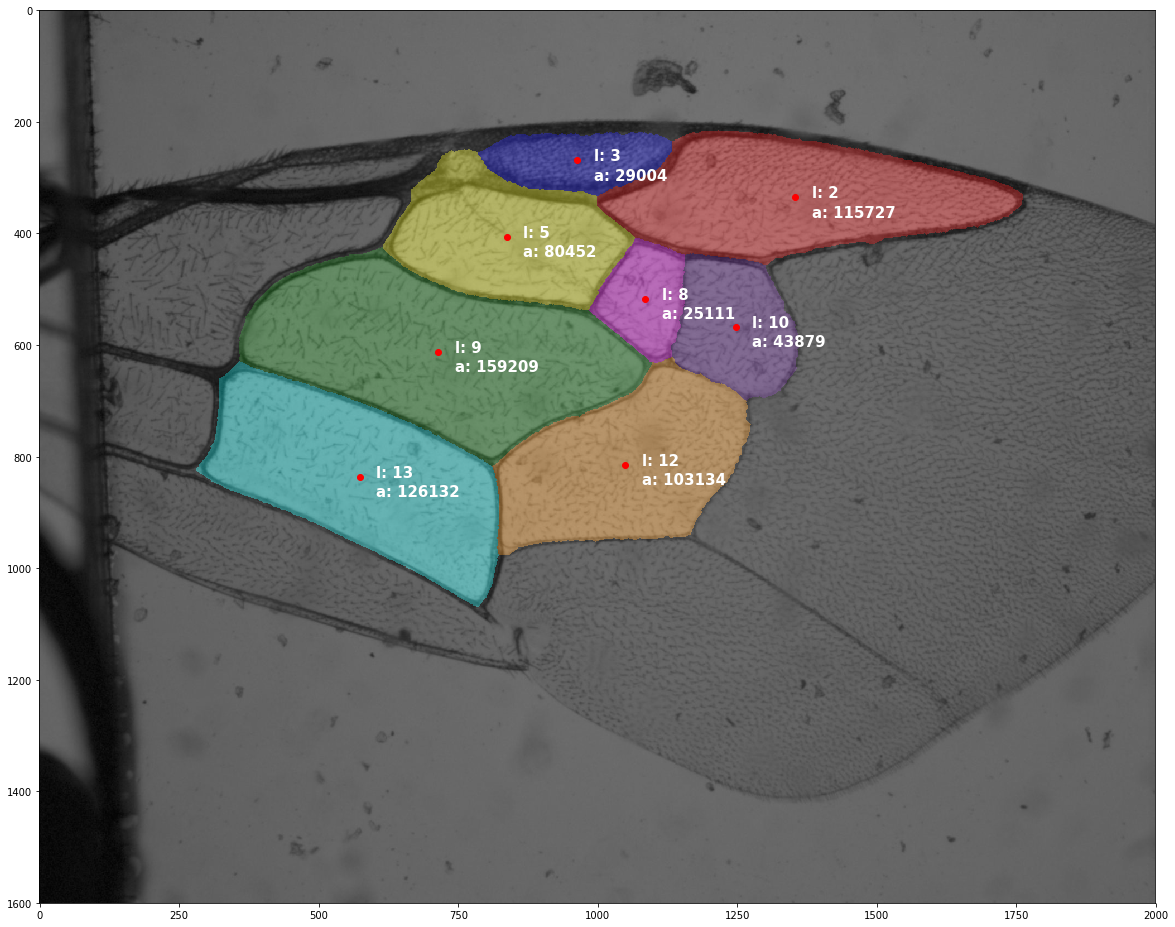
\includegraphics[width=.6\textwidth]{figures/filter_neighbors.png}
    \caption{Filter neighbors}
\end{figure}

\subsubsection{Central cell}

To continue the precess pf selection, we need a cell of reference that we call "central cell", whiwh corresponds to the first submarginal cell. 
To find it, we compute a score for each region : $score = area * neighbors$
For better accuracy, we also dismiss regions that are too eccentric to be the central cell. 

\begin{figure}[H]
    \centering
    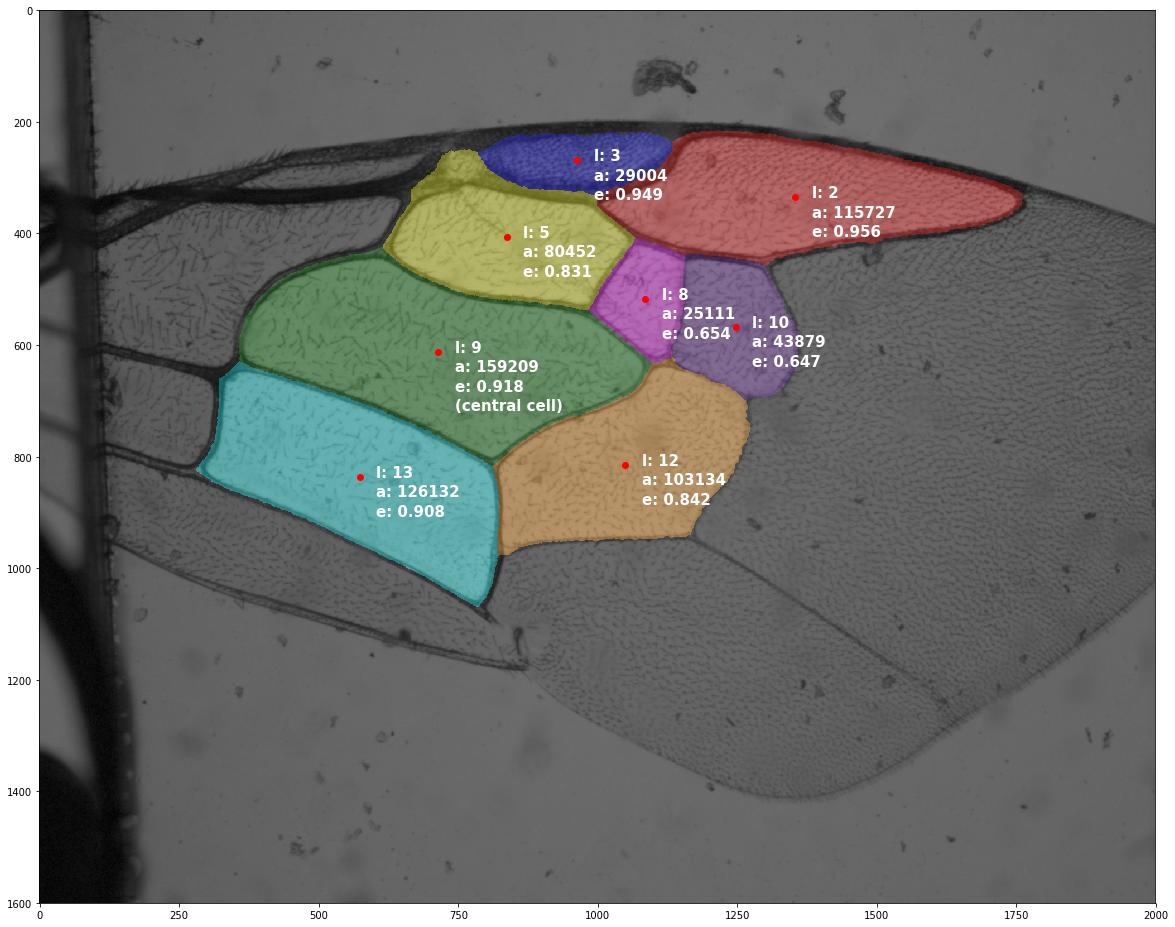
\includegraphics[width=.6\textwidth]{figures/central_cell.png}
    \caption{Central cell found}
    \label{central_cell}
\end{figure}

As shown on figure \ref{central_cell}, the central cell as been correctly found and labeled.


\subsubsection{Angles filters}

\begin{figure}[H]
\begin{subfigure}{.5\textwidth}
    \centering
    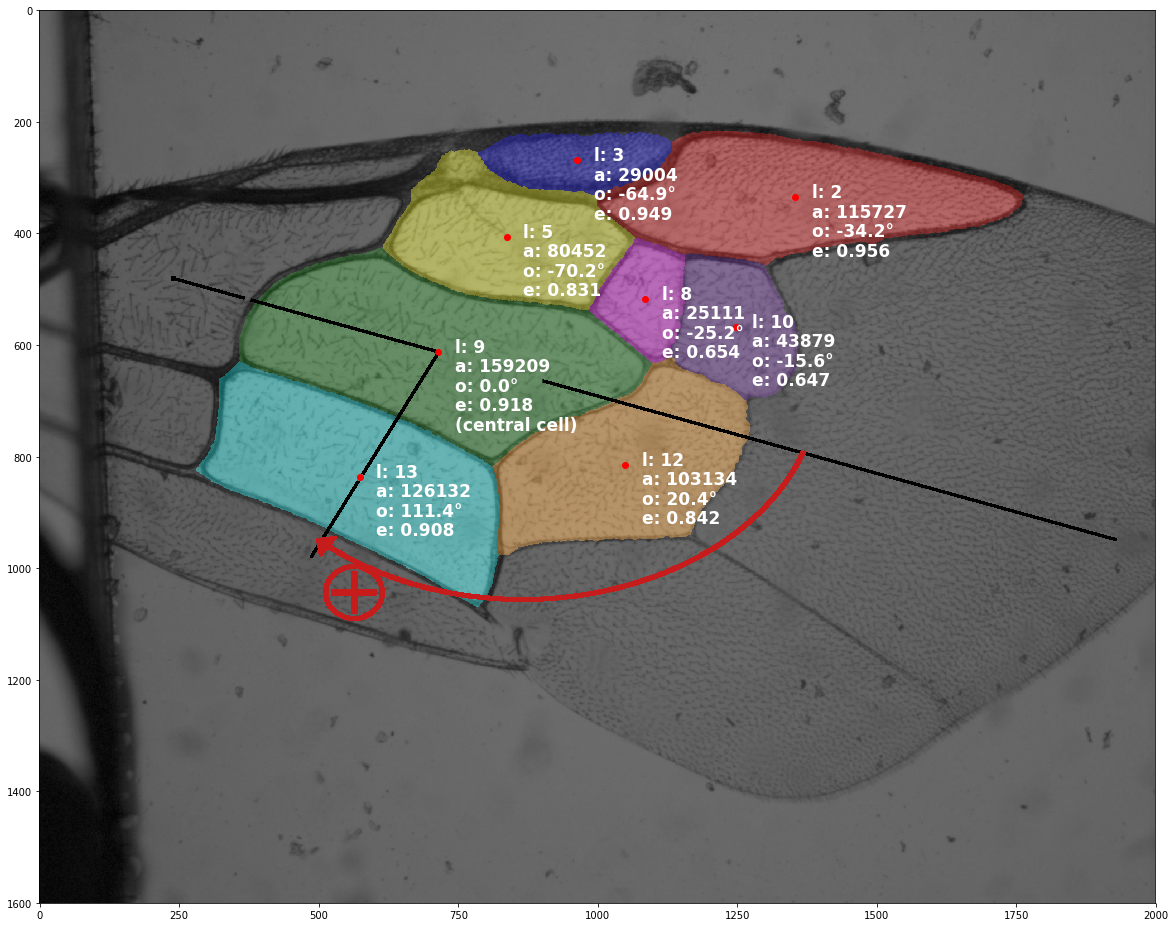
\includegraphics[width=\linewidth]{figures/angles2.png}
    \caption{Computing angles}
\end{subfigure}
\begin{subfigure}{.5\textwidth}
    \centering
    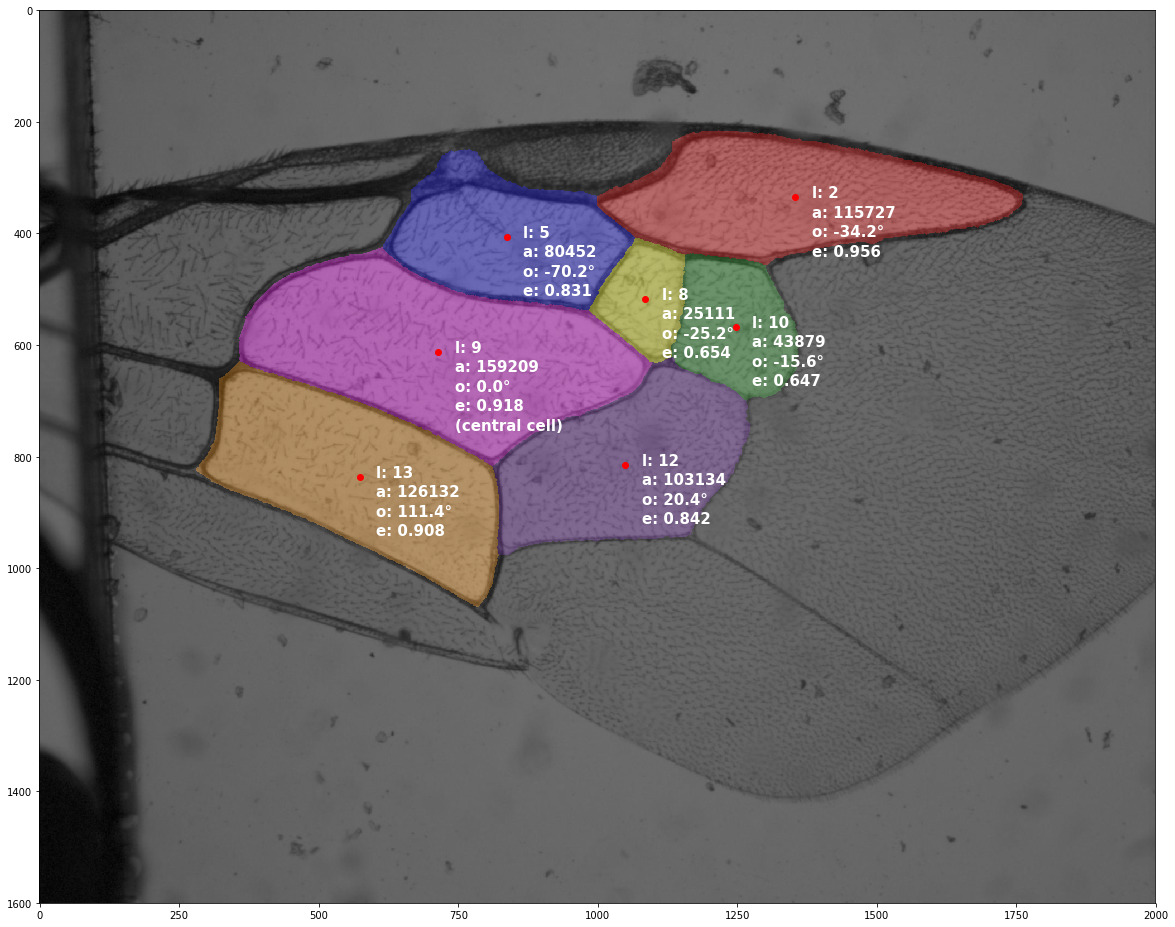
\includegraphics[width=\linewidth]{figures/filter_angle.png}
    \caption{After angle filtering}
\end{subfigure}
\caption{Angles filter}
\end{figure}

Now that we have a point of reference, we can determine angles of other regionswith respect to the central cell. We first compute the orientation of the central cell, then we can find the angle between : the centroid of the focused region, the central cell's centroid, and the central cell's orientation. 

Then we will discard regions based on their angle and their proximity to the central cell :
\begin{itemize}
    \item Direct neighbors of the central must have an angle ranging from -80° to 150°
    \item Degree 2 neighbors must have an angle ranginf from -40° to 5°
    \item Other regions are discarded
\end{itemize}

\subsection{Cells identification}

Now we should have 6 or 7 regions remaining, depending on the species. If not, the image is discarded as invalid.
We use the angles and their proximity to the central cell to label them, the result is shown in figure \ref{identify}.

\begin{figure}[H]
    \centering
    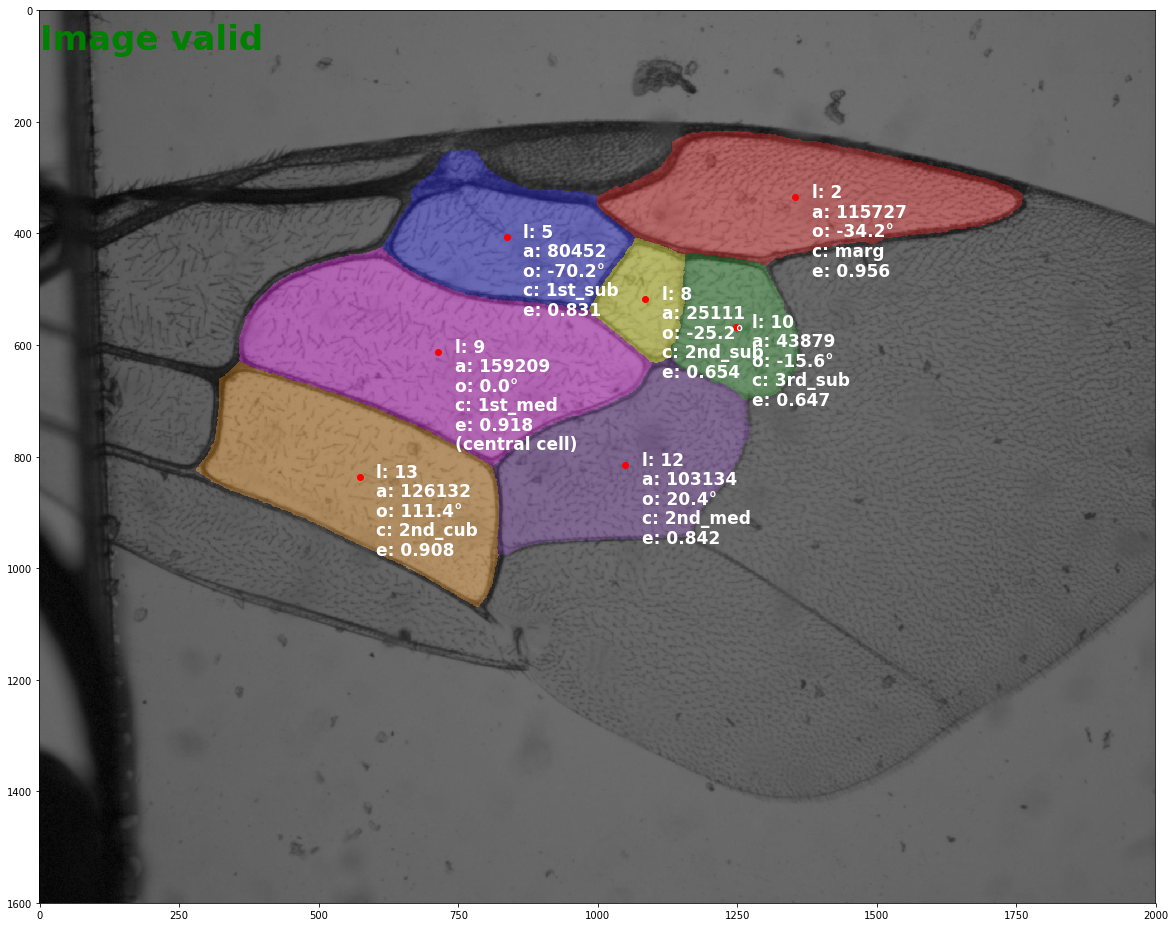
\includegraphics[width=\textwidth]{figures/identify_regions.png}
    \caption{Identified regions}
    \label{identify}
\end{figure}


\subsection{Features extraction}

Now that our cells are indentified and labeled, we can extract features from them that will be used for classification.

\subsubsection{Fourier descriptors}

For each cell, we compute the Fourier descriptors, which contain information about the overall cell's shape.
To do so, we first compute the boudnary of each cell using the Moore neighboroog algorithm, and then we use Fourier tranformation to keep only the first coefficients.

\begin{figure}
    \begin{subfigure}{0.45\textwidth}
  \centering
    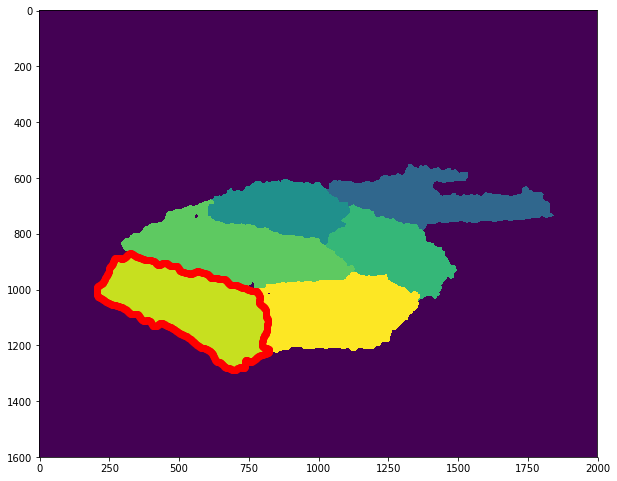
\includegraphics[width=\linewidth]{figures/boundary.png}
        \caption{Boundary tracing: Moore neighborhood}
    \end{subfigure}
\begin{subfigure}{0.45\textwidth}
  \centering
    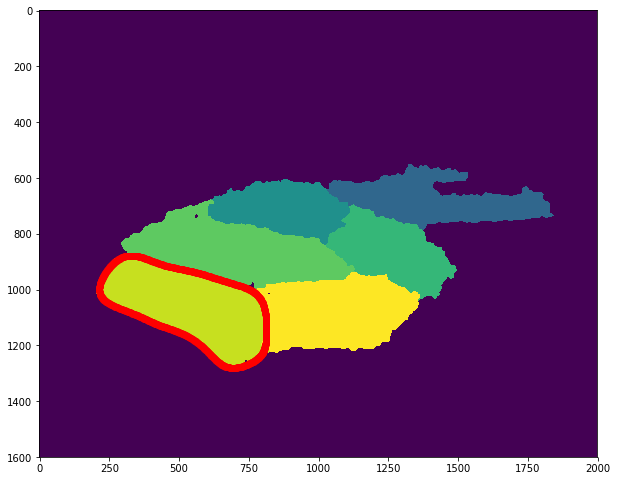
\includegraphics[width=\linewidth]{figures/fourier.png}
    \caption{Inverse Fourier transformation}
    \end{subfigure}
    \caption{Extraction of the first 15 Fourier descriptors}

\end{figure}


\noindent\textbf{Fourier descriptors:}\\
    Let $x[m]$ and $y[m]$ be the coordinates of the mth pixel on the boundary of a given 2D shape containing $N$ pixels, a complex number can be formed as  $z[m]=x[m]+jy[m]$\\
    $$\forall k \in\scalebox{0.85}[1.0]{[0, 1, -1, .. N-1, -(N-1)]}, \quad Z[k] = \frac{1}{N}\displaystyle\sum_{m=0}^{N-1} z[m]e^{-j2\pi mk/N}$$
\textbf{Inverse transformation:}\\
To reconstruct the signal from the first $M$ Fourier descriptors :
    $$\forall m \in \scalebox{0.85}[1.0]{[\![0, N-1]\!]}, \quad \hat{z}[m] = \displaystyle\sum_{k=-M/2}^{M/2} Z[k]e^{-j2\pi mk/N}$$


\subsubsection{Results features extraction}
For each cell, we extract the following features:
    \begin{itemize}
        \item area (scaled with the total area of detected cells)
        \item eccentricity
        \item angle with respect to the central cell
        \item first 15 normalized Fourier descriptors
    \end{itemize}
    \vspace{3pt}
\large{\textbf{Results of cells detection:}}\\
    \vspace{15pt}
\begin{tabular}{ |m{2cm}|m{10em}|m{8em}| }
 \hline
category & Features extraction & Groundtruth \\
\hline
invalid & 101 (9\%) &  0\\
valid & 1034 (91\%)  & 1135 (100\%)\\
\hline
\end{tabular}

We then applied a Random Forest classifier on the valid dataset, which had a 83\% accuracy on test set (and 100\% on training set).

\newpage
\section{Conclusion}

\begin{figure}[h]
    \centering
    \begin{tabular}{ |c|c|c| }
 \hline
Model & training accuracy & test accuracy\\
\hline
DenseNet121& 99\% & 95\%\\
\hline
VGG16& 98\% & 88\%\\
\hline
    \makecell{Features extraction + \\Random Forest \\(on valid dataset)}& 100\% & 83\% \\
\hline
\end{tabular}
\caption{Models comparison}
\end{figure}

We can see the CNN models remain more accurate than features extraction + random forest with out method, at the cost of a heavier model. Furthermore, no features engineering is required with CNN, whichh is a huge advantage in such a project. 
\end{document}
